\documentclass{beamer}
\usetheme{Copenhagen}
\usepackage[utf8]{inputenc}


%\usepackage{graphicx}
%\usepackage{subfigure}
%\usepackage{multimedia}
\usepackage{times}  % fonts are up to you
\usepackage{graphics}
\usepackage{amsmath}
\usepackage{media9}
\usepackage{hyperref}
\usepackage{psfrag}
\usepackage{pdfpages}
\usepackage{tikz}
\usepackage{listings}
%\usepackage[style=authoryear]{biblatex}
%\bibliography{/Users/ali/Library/texmf/bibtex/bib/references}


\setbeamertemplate{bibliography item}[text]
%\usepackage[backend=bibtex, style=authoryear]{biblatex}
%\addbibresource{/Users/ali/Library/texmf/bibtex/bib/references.bib}
\newcommand{\customcite}[1]{\citeauthor{#1}, \citeyear{#1}}
\newcommand\smallFont{\fontsize{8}{7.2}\selectfont}   %Change font size.
\newcommand\mCite[1]{[\cite{#1}, \citetitle{#1}]}  %Prints name and title
\newcommand\FrameText[1]{
\begin{textblock*}{\paperwidth}(0pt,\textheight)
	\vspace{1.0cm}
    \raggedleft \smallFont #1
\end{textblock*}}

% https://tex.stackexchange.com/a/61016/84495
\newcommand{\chref}[3][blue]{\href{#2}{\color{#1}{#3}}}%

%Get rid of ugly copenhagen default symbol for enumerate
\setbeamertemplate{enumerate items}[default]   


% Create code text
% https://tex.stackexchange.com/questions/65291/code-snippet-in-text
\definecolor{codegray}{gray}{0.9}
\newcommand{\code}[1]{\colorbox{codegray}{\texttt{#1}}}




%Information to be included in the title page:
\title{Introduction to Linux and HPC for Bioinformaticians }
\author{Ali Snedden}
\institute{Nationwide Children's Hospital}
\date{March 17, 2022}
 
% Recurring Outline
\AtBeginSection[]  % "Beamer, do the following at the start of every section"
{
\begin{frame}<beamer>
\frametitle{Outline} % make a frame titled "Outline"
\tableofcontents[currentsection]  % show TOC and highlight current section
\end{frame}
}
 
 
\begin{document}
 
\frame{\titlepage}

\section{Introduction}

\begin{frame}
\frametitle{What is Linux?}
\begin{itemize}
    \item It is an Operating System, just like Mac OS and Windows  
    \pause 
    \item It is EVERYWHERE
    \begin{enumerate}
        \item Billions of Android phones 
        \pause 
        \item `Smart' home devices 
        \pause 
        \item Millions of cloud servers
        \begin{enumerate}
            \item AWS (Amazon Web Services)
            \pause
            \item Google Cloud.
        \end{enumerate}
        \pause 
        \item It runs the world's most `cutting edge' scientific experiments
    \end{enumerate}
\end{itemize}
\end{frame}


\begin{frame}
\frametitle{Linux in Science}
\begin{picture}(320,250)
\visible<1>{\put(165, 100){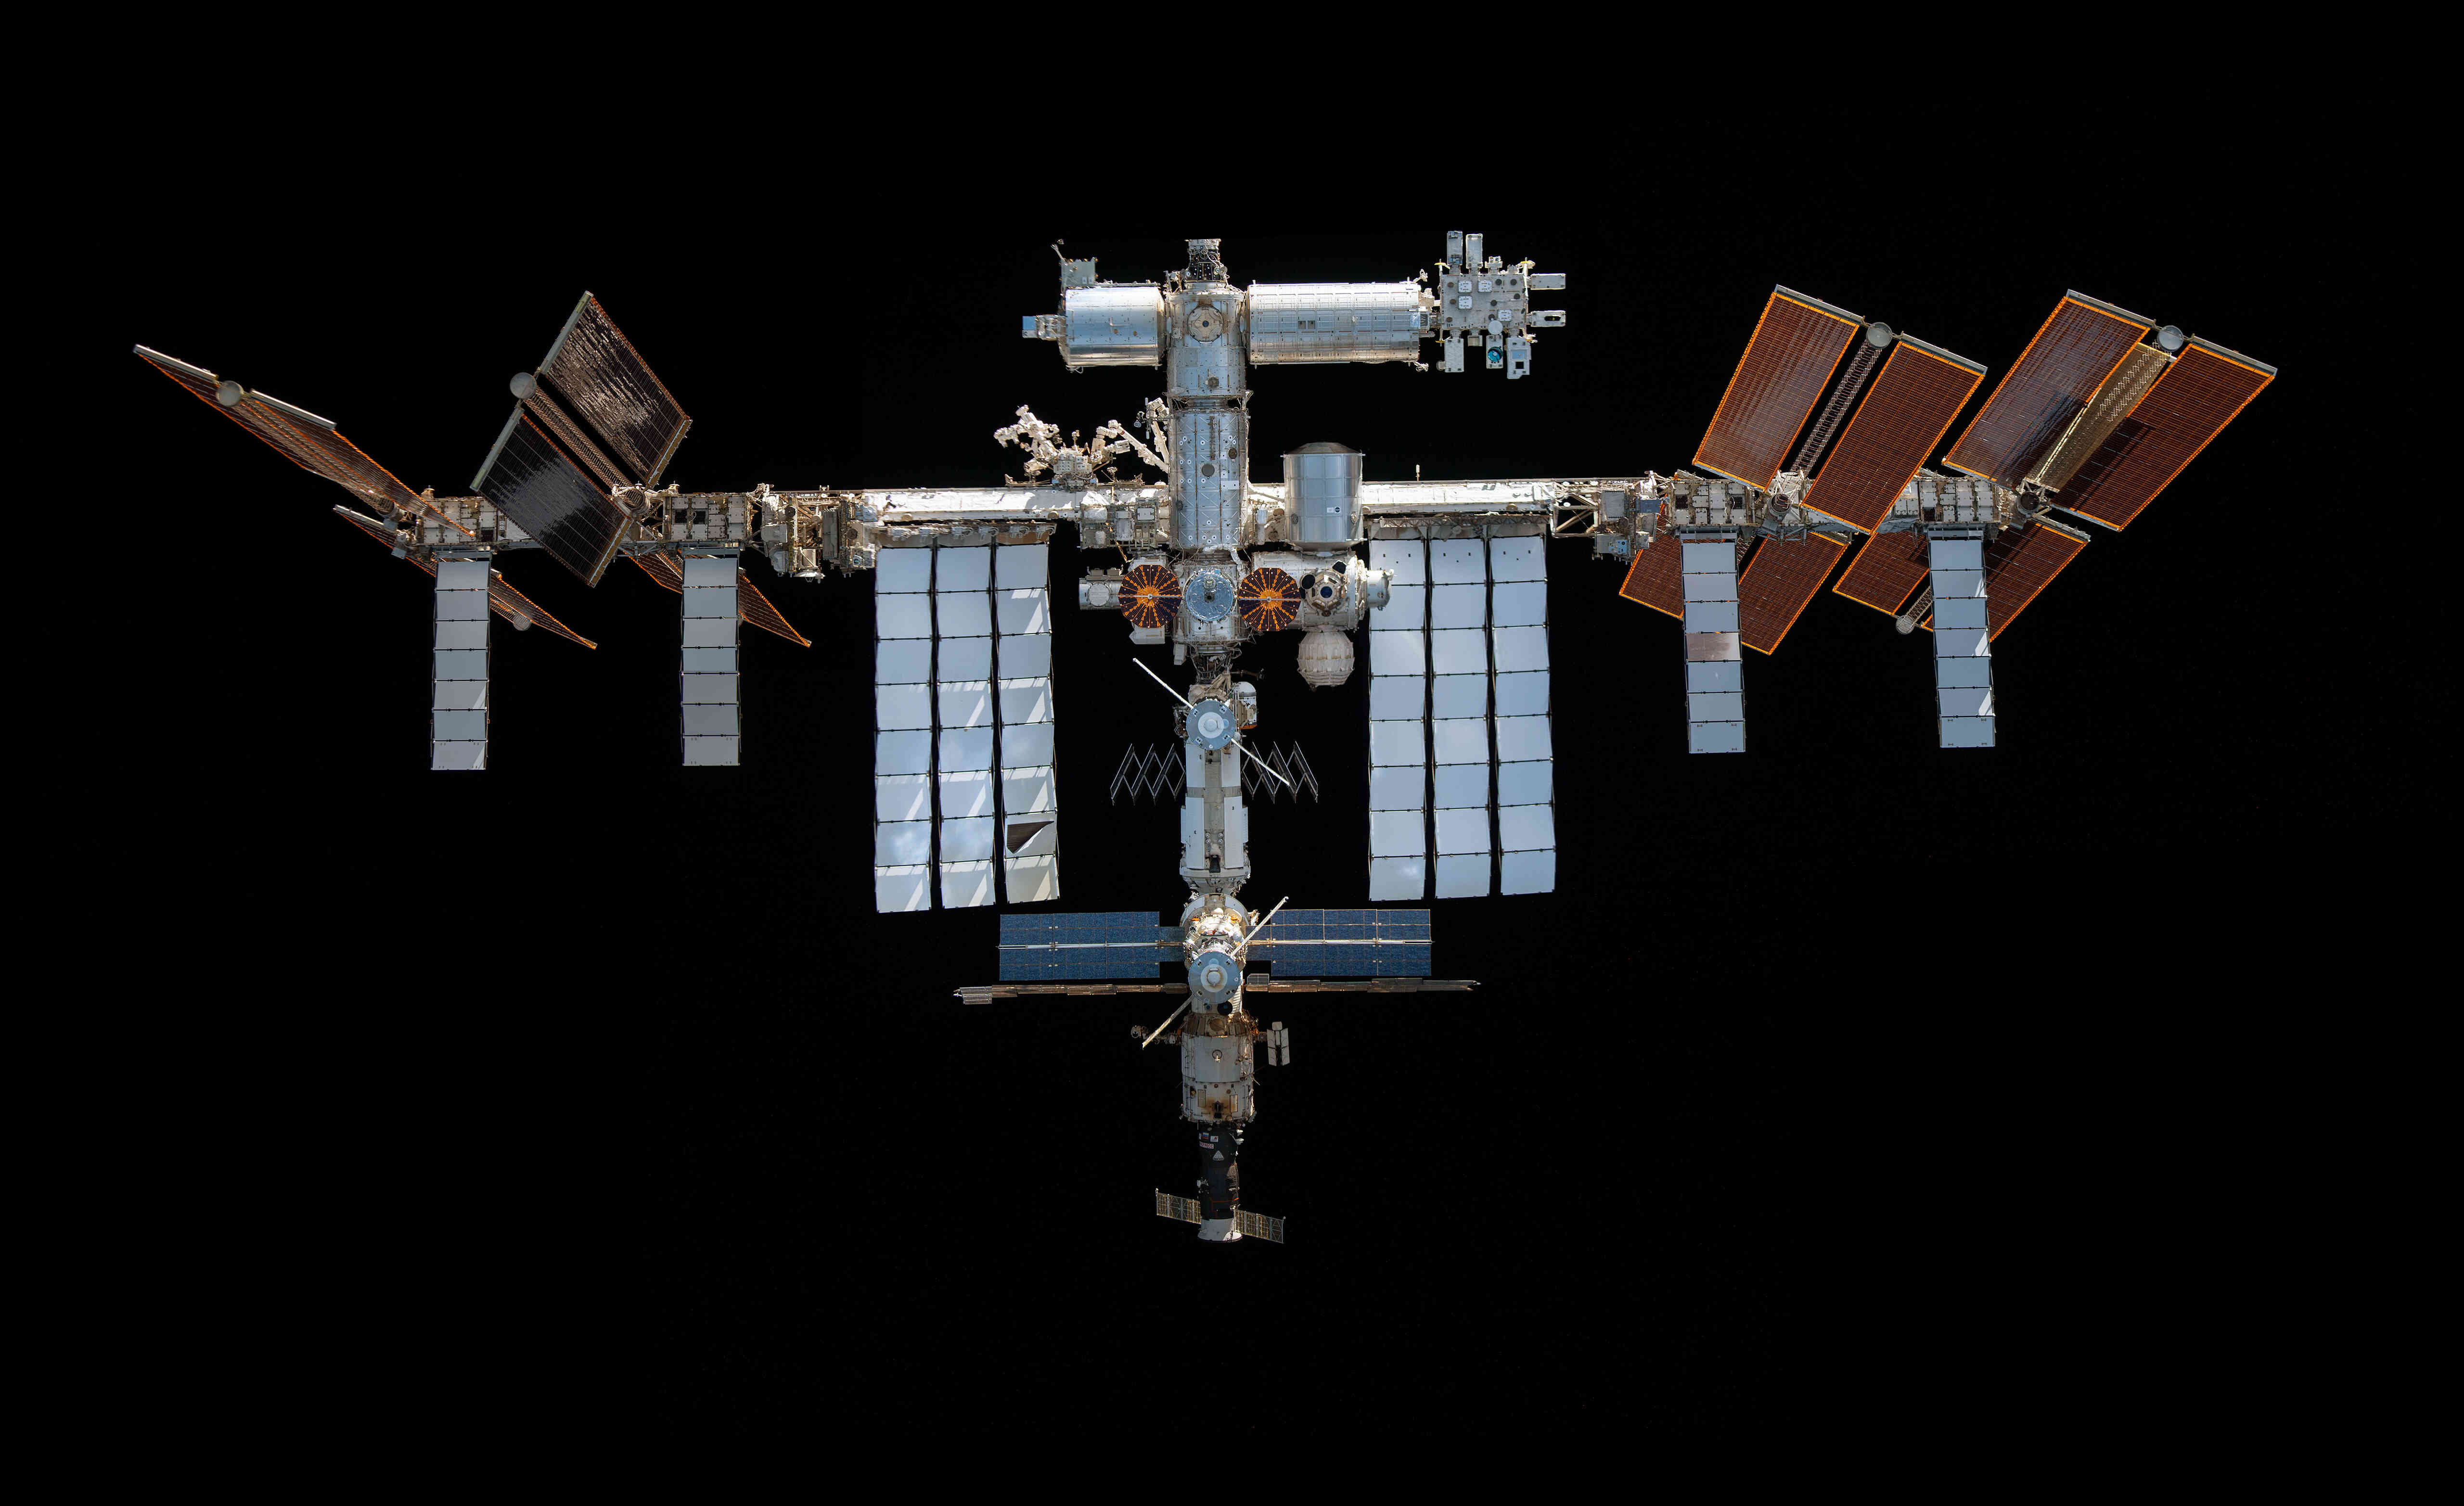
\includegraphics[height=1.5in]{images/spacestationfaqs-small.jpg}}}
\visible<2>{\put(165, 100){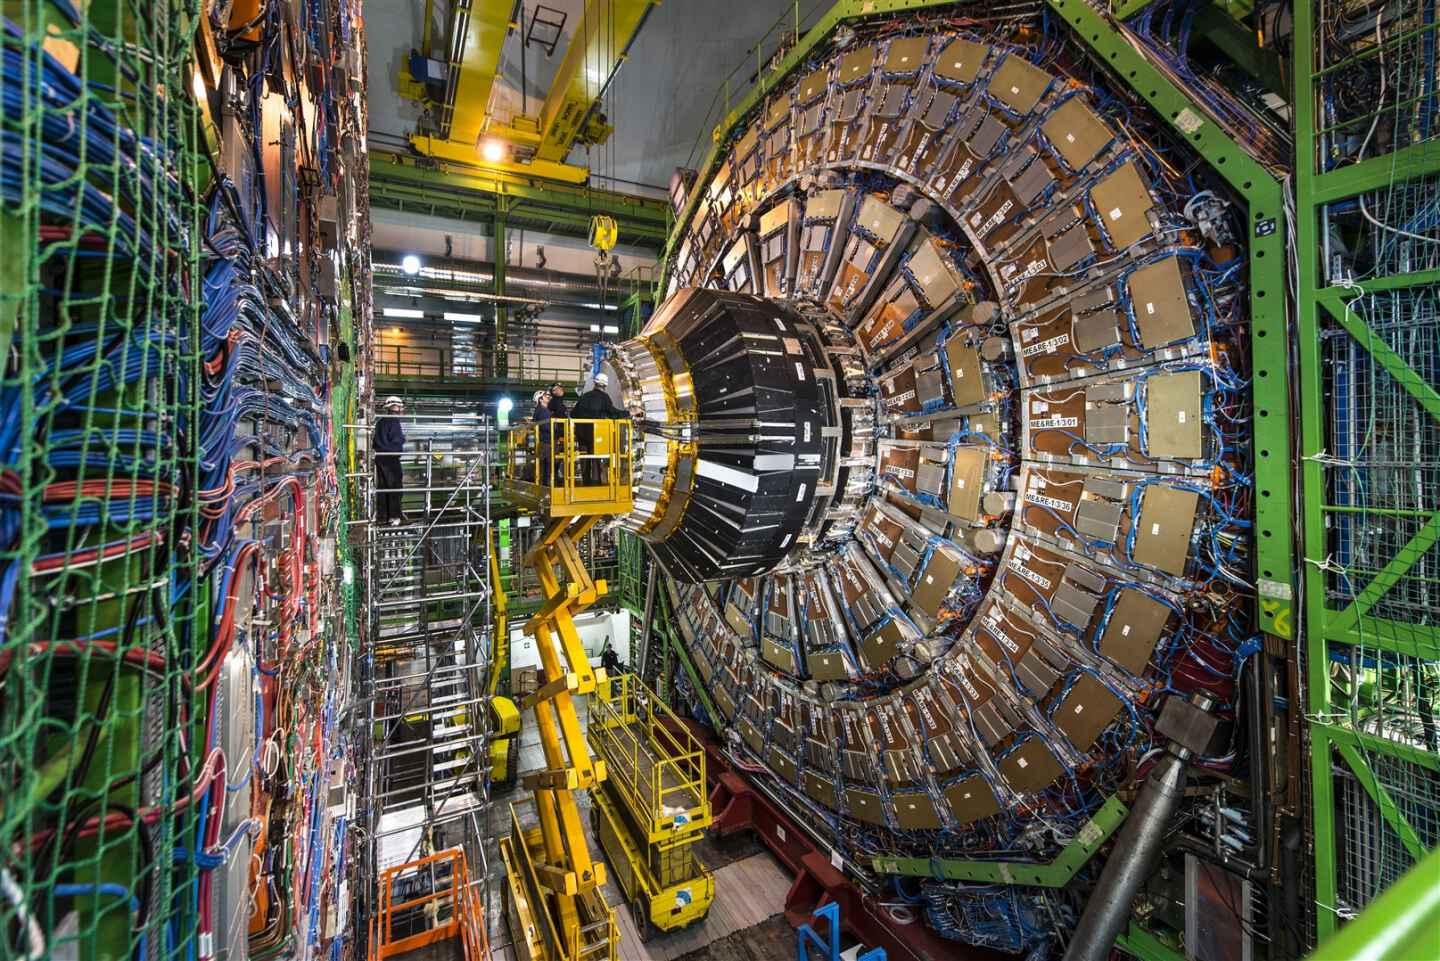
\includegraphics[height=1.5in]{images/LHC-small.jpg}}}
\visible<3>{\put(165, 100){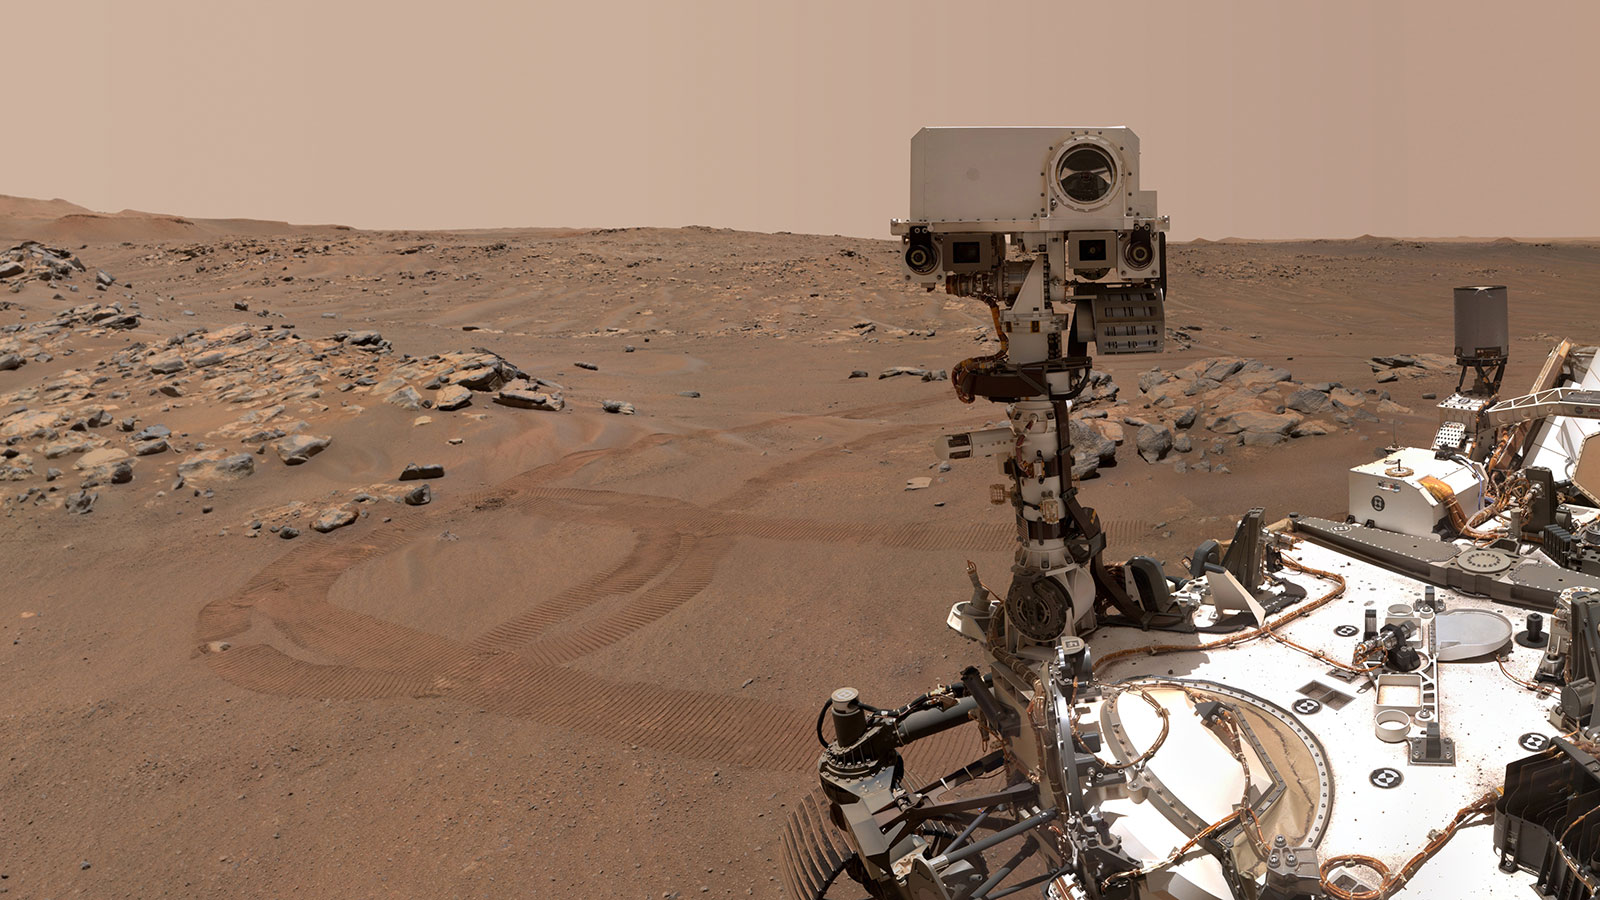
\includegraphics[height=1.5in]{images/perserverance.jpg}}}
\visible<4>{\put(205, 100){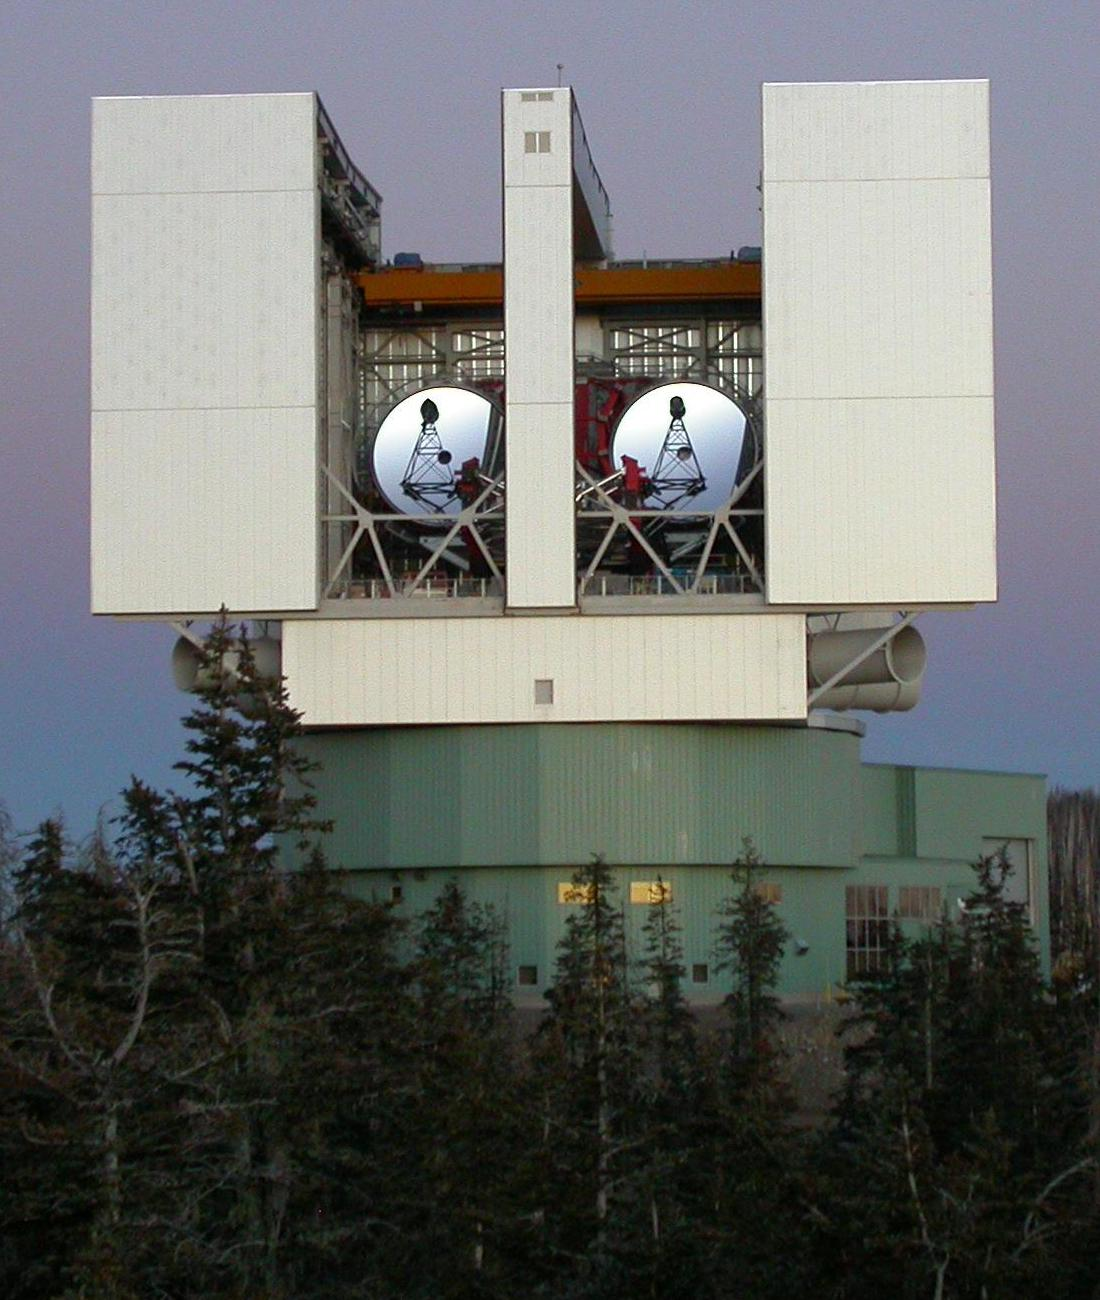
\includegraphics[height=1.5in]{images/LBT.jpg}}}
\visible<5>{\put(165, 100){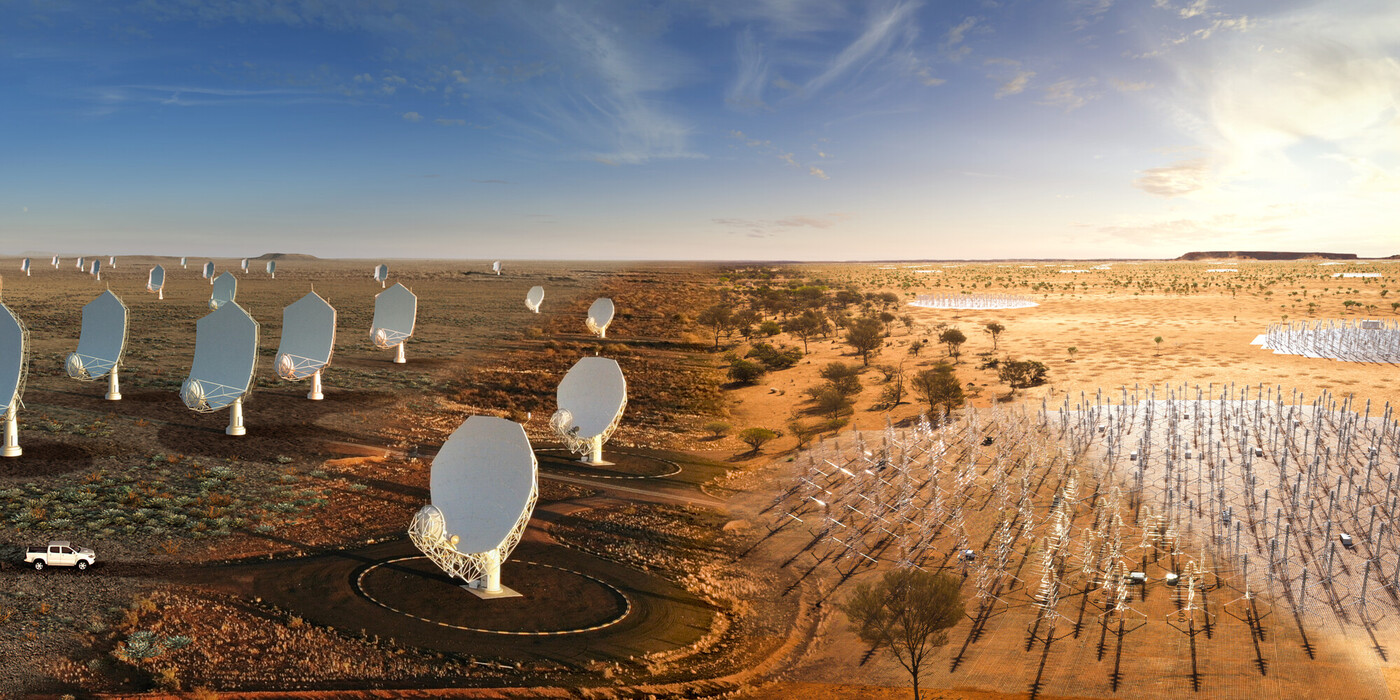
\includegraphics[height=1.5in]{images/ska.jpg}}}
\visible<6>{\put(165, 70){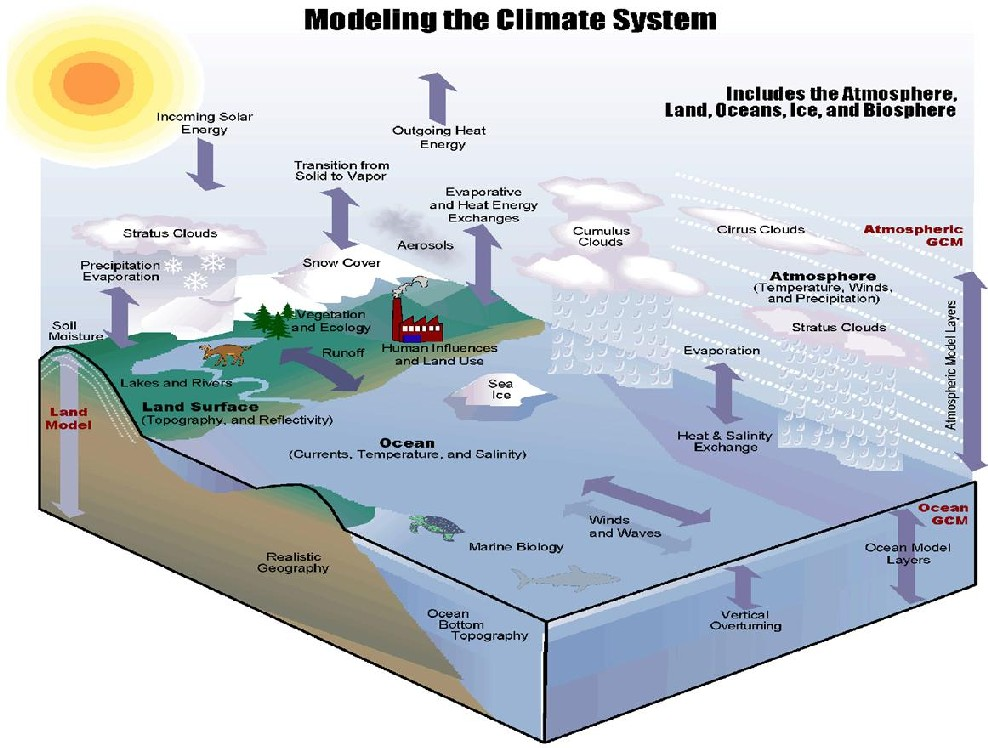
\includegraphics[height=1.75in]{images/climate.jpg}}}
\put(-20, 220){\begin{minipage}[t]{0.6 \linewidth}
{
Linux in Science : 
\begin{itemize}
    { \small
    \item International Space Station
    \smallskip
    \pause
    \item CERN's Large Hadron Collider 
    \begin{itemize}
        \item[-] Higg's boson 
    \end{itemize}
    \smallskip
    \pause
    \item Perseverance on Mars
    \begin{itemize}
        \item[-] Ingenuity, the Mars Helicopter
    \end{itemize}
    \smallskip
    \pause
    \item Large Binocular Telescope
    \smallskip
    \pause
    \item Square Kilometer Array 
    \begin{itemize}
        \item[-] Processing 600PB per year
    \end{itemize}
    \smallskip
    \pause
    \item Climate Simulations 
    }
\end{itemize}
}
\end{minipage}}
\end{picture}
\end{frame}


%\begin{frame}
%\frametitle{Why use Linux?}
%\begin{itemize}
%    \item Package managers (e.g. \code{yum})
%    \bigskip
%    \item Built for programming. Comes with compilers, editors etc.
%    \bigskip
%    \item Great online resources (e.g. https://stackoverflow.com/)
%    \bigskip
%    \item Customizable
%    \bigskip
%    \item Dominant HPC platform.
%\end{itemize}
%\end{frame}


\begin{frame}
\frametitle{Why use Linux?}
Two perspectives : 
\begin{itemize}
    \item System Administrator / Power user
    \pause
    \begin{enumerate}
        \item Open Source 
        \begin{itemize}
            \pause
            \item[-] Many eyes on source code ensures quality
        \end{itemize}
        \pause
        \item High Security 
        \pause
        \item High Stability
        \begin{itemize}
            \pause
            \item[-] e.g. CentOS 7.X has a 10 year lifespan
            \pause
            \item[-] Installing new software doesn't require reboot
        \end{itemize}
        \pause
        \item Easy to Manage
        \begin{itemize}
            \pause
            \item[-] There aren't barriers to getting work done, i.e. ``autocorrect"
            \pause
            \item[-] The OS doesn't take the attitude that the user is an idiot.
            \pause
            \item[-] Very mature command line interface with powerful tools like \code{grep}, \code{find}, \code{crontab}
        \end{itemize}
        \pause
        \item Availability of Software
        \pause
        \begin{itemize}
            \item[-] Vast majority of scientific software was developed on Linux 
            \pause
            \item[-] Most scientific software on Linux is Open Source 
        \end{itemize}
    \end{enumerate}
\end{itemize}
\end{frame}


\begin{frame}
\frametitle{Why use Linux?}
\begin{itemize}
    \item Personal user
    \pause
    \begin{enumerate}
        \item Built for programming
        \begin{itemize}
            \pause
            \item[-] vi / vim / emacs
            \pause
            \item[-] powerful debuggers (e.g. \code{pdb}, \code{gdb})
            \pause
            \item[-] containers (e.g. Singularity)
        \end{itemize}
        \pause
        \item Can run on old / underpowered hardware
        \begin{itemize}
            \item[-] Raspberry Pi is a \$35 computer
        \end{itemize}
        \pause
        \item Free : cost = \$0, 
        \pause
        \begin{itemize}
            \item[-] free as in beer
        \end{itemize}
        \pause
        \item Open Source 
        \begin{itemize}
            \pause
            \item[-] Free as in freedom 
            \pause
            \item[-] You can change the OS code (i.e. free as in freedom)
        \end{itemize}
    \end{enumerate}
\end{itemize}
\end{frame}


\begin{frame}
\frametitle{Why use Linux?}
\begin{itemize}
    \item Personal user
    \begin{enumerate}
        \pause
        \item Highly customizable
        \begin{itemize}
            \pause
            \item[-] You can configure your environment how you want to in a transparent way
        \end{itemize}
        \pause
        \item Support - strong user community
        \begin{itemize}
            \item[-] https://stackoverflow.com/
            \pause
            \item[-] https://unix.stackexchange.com/
        \end{itemize}
        \pause
        \item Stability
        \begin{itemize}
            \pause
            \item[-] No `convenient' forced reboots to update / upgrade the OS.
        \end{itemize}
        \pause
        \item Security, Safety and Privacy
        \begin{itemize}
            \pause
            \item[-] No NSA keys
            \pause
            \item[-] You won't become a monetized consumer product by your OS.
        \end{itemize}
        \pause
        \item All High Performance Computing (HPC) clusters use Linux
    \end{enumerate}
\end{itemize}
\end{frame}


\begin{frame}
\frametitle{What is HPC?}
\begin{itemize}
    \item Q : What is High Performance Computing (HPC)?
    \pause
    \item A : A collection of computers connected on a high speed network with
              shared storage that specialize in distributed / parallel computing
    \pause
    \bigskip
    \item Q : What is High Performance Computing good for?
    \pause
    \item A : Solving problems too big to solve on your desktop or laptop computers.
    \pause
    \bigskip
    \item Q : What is ``parallel computing"?
    \pause
    \item A : It is breaking up independent tasks and running them simultaneously so they complete faster.
    \bigskip
\end{itemize}
\end{frame}


\begin{frame}
\frametitle{What is HPC?}
\begin{itemize}
    \item Q : What some examples of HPC type problems in the life sciences?
    \pause
    \item A : Examples : 
    \pause
    \begin{enumerate}
        \item Aligning dozens of fastq files to the human genome at the same time
        \pause
        \item Reconstructing medical images (e.g. CT, MRI) in real time
        \pause
        \item Image analysis of bacteria films
        \pause
        \item Modelling biological systems at the individual cell level
        \pause
        \item Genetic linkage analysis
        \pause
        \item Protein folding 
        \pause
        \item Machine Learning
    \end{enumerate}
\end{itemize}
\end{frame}



\begin{frame}
\frametitle{How to Connect}
Windows:
\begin{itemize}
    \item Open PuTTY
    \item Window Session $\Rightarrow$ Host Name field : username@r1pl-hpcf-log01
    \item Click ``Open" to log in.
    \item Enter password
\end{itemize}

\pause

Mac:
\begin{itemize}
    \item Open Terminal (Finder $\Rightarrow$ Utilities $\Rightarrow$ Terminal)
    \item \code{ssh -X username@r1pl-hpcf-log01}
\end{itemize}
\end{frame}

\begin{frame}
\frametitle{How to Connect}
eChart:
\begin{itemize}
    \item Go to: nchapps.nationwidechildrens.org/
    \pause
    \item Click on ‘Desktops’ at top
    \pause
    \item Click on eChart Connect Desktop-Win10
    \pause
    \item Click finder magnifying glass. Search for HPC
    \pause
    \item Click XLaunch. Click Next / Finish for all following windows.  A little ‘x’ will
          be at the bottom right of your screen
    \pause
    \item Click finder magnifying glass. Search for HPC.
    \pause
    \item Click Putty. 
    \pause
    \begin{enumerate}
        \item Host Name = r1pl-hpcf-log01
        \pause
        \item Check Connection$\rightarrow$ SSH $\rightarrow$ X11 $\rightarrow$ Enable X11 forwarding. 
        \pause
        \item Check Connection$\rightarrow$ SSH $\rightarrow$ Enable compression
        \pause
        \item Click "Open"
        \pause
        \item Enter your userID and password when prompted
    \end{enumerate}
\end{itemize}
\end{frame}


%\begin{frame}
%\frametitle{What is Linux?}
%Operating System
%\begin{itemize}
%    \item Bootloader 
%    \item Kernel - interface between the hardware and operating system. Manages processes.
%    \item Daemons - background processes
%    \item Graphical Interface -  X11 or X
%    \item Shell - a.k.a. ``The Command Line".  This will be where you interface with Linux.
%\end{itemize}
%\end{frame}
 
\section{Linux}

\begin{frame}
\frametitle{Types of Users}
\begin{itemize}
    \item Regular users (you)
    \bigskip
    \pause
    \item Privileged users (Yuan and myself)
    \bigskip
    \pause
    \begin{enumerate}
        \item Can modify \code{/usr}, \code{/opt}, etc.
        \bigskip
        \pause
        \item \code{sudo}
    \end{enumerate}
\end{itemize}
\end{frame}


\begin{frame}
\frametitle{The ``Shell"}
   \begin{picture}(320,250)  %must be related to where it is centered
    \visible<1-3>{\put(165, 80){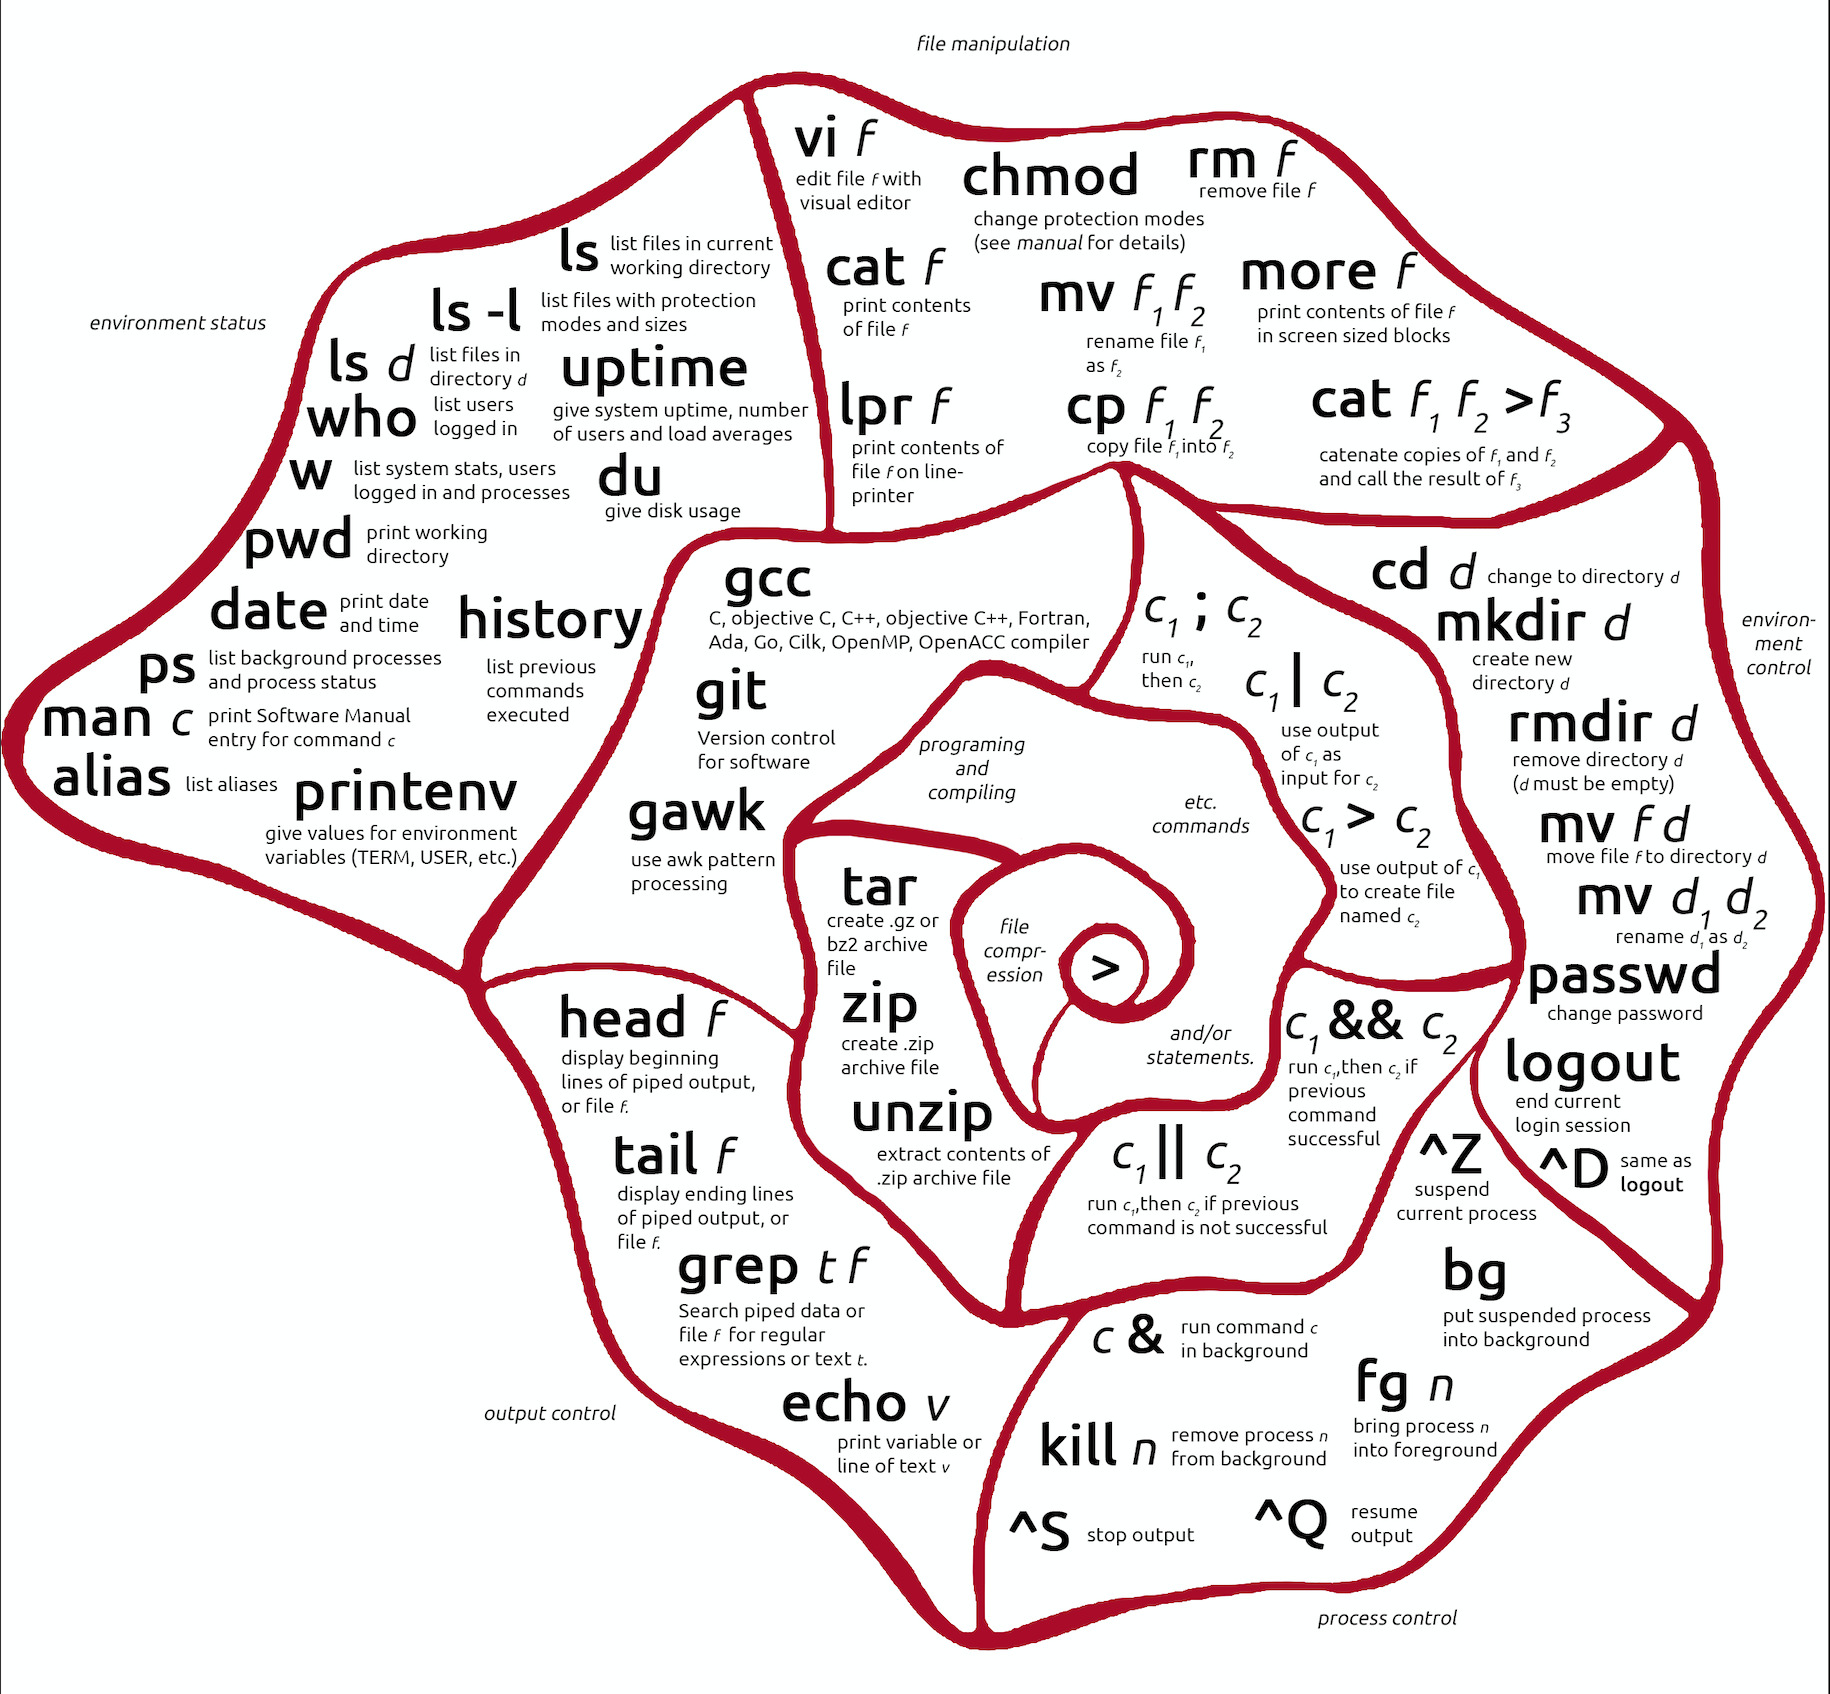
\includegraphics[height=2.2in]{images/linux-shell-small.jpg}}}
    \put(-20, 220){\begin{minipage}[t]{0.6 \linewidth}
    {
    \begin{itemize}
        \item Used at the command line, i.e. the `terminal'
        \pause
        \bigskip
        \item The user interface with the operating system
        \pause
        \bigskip
        \item Bash is the default shell on Franklin.
    \end{itemize}
    }
    \end{minipage}}
    %\put(0, 70){\includegraphics[height=2.5in]{images/GPFS_File.eps}}
    %\setbeamercolor{background canvas}{bg=}
    %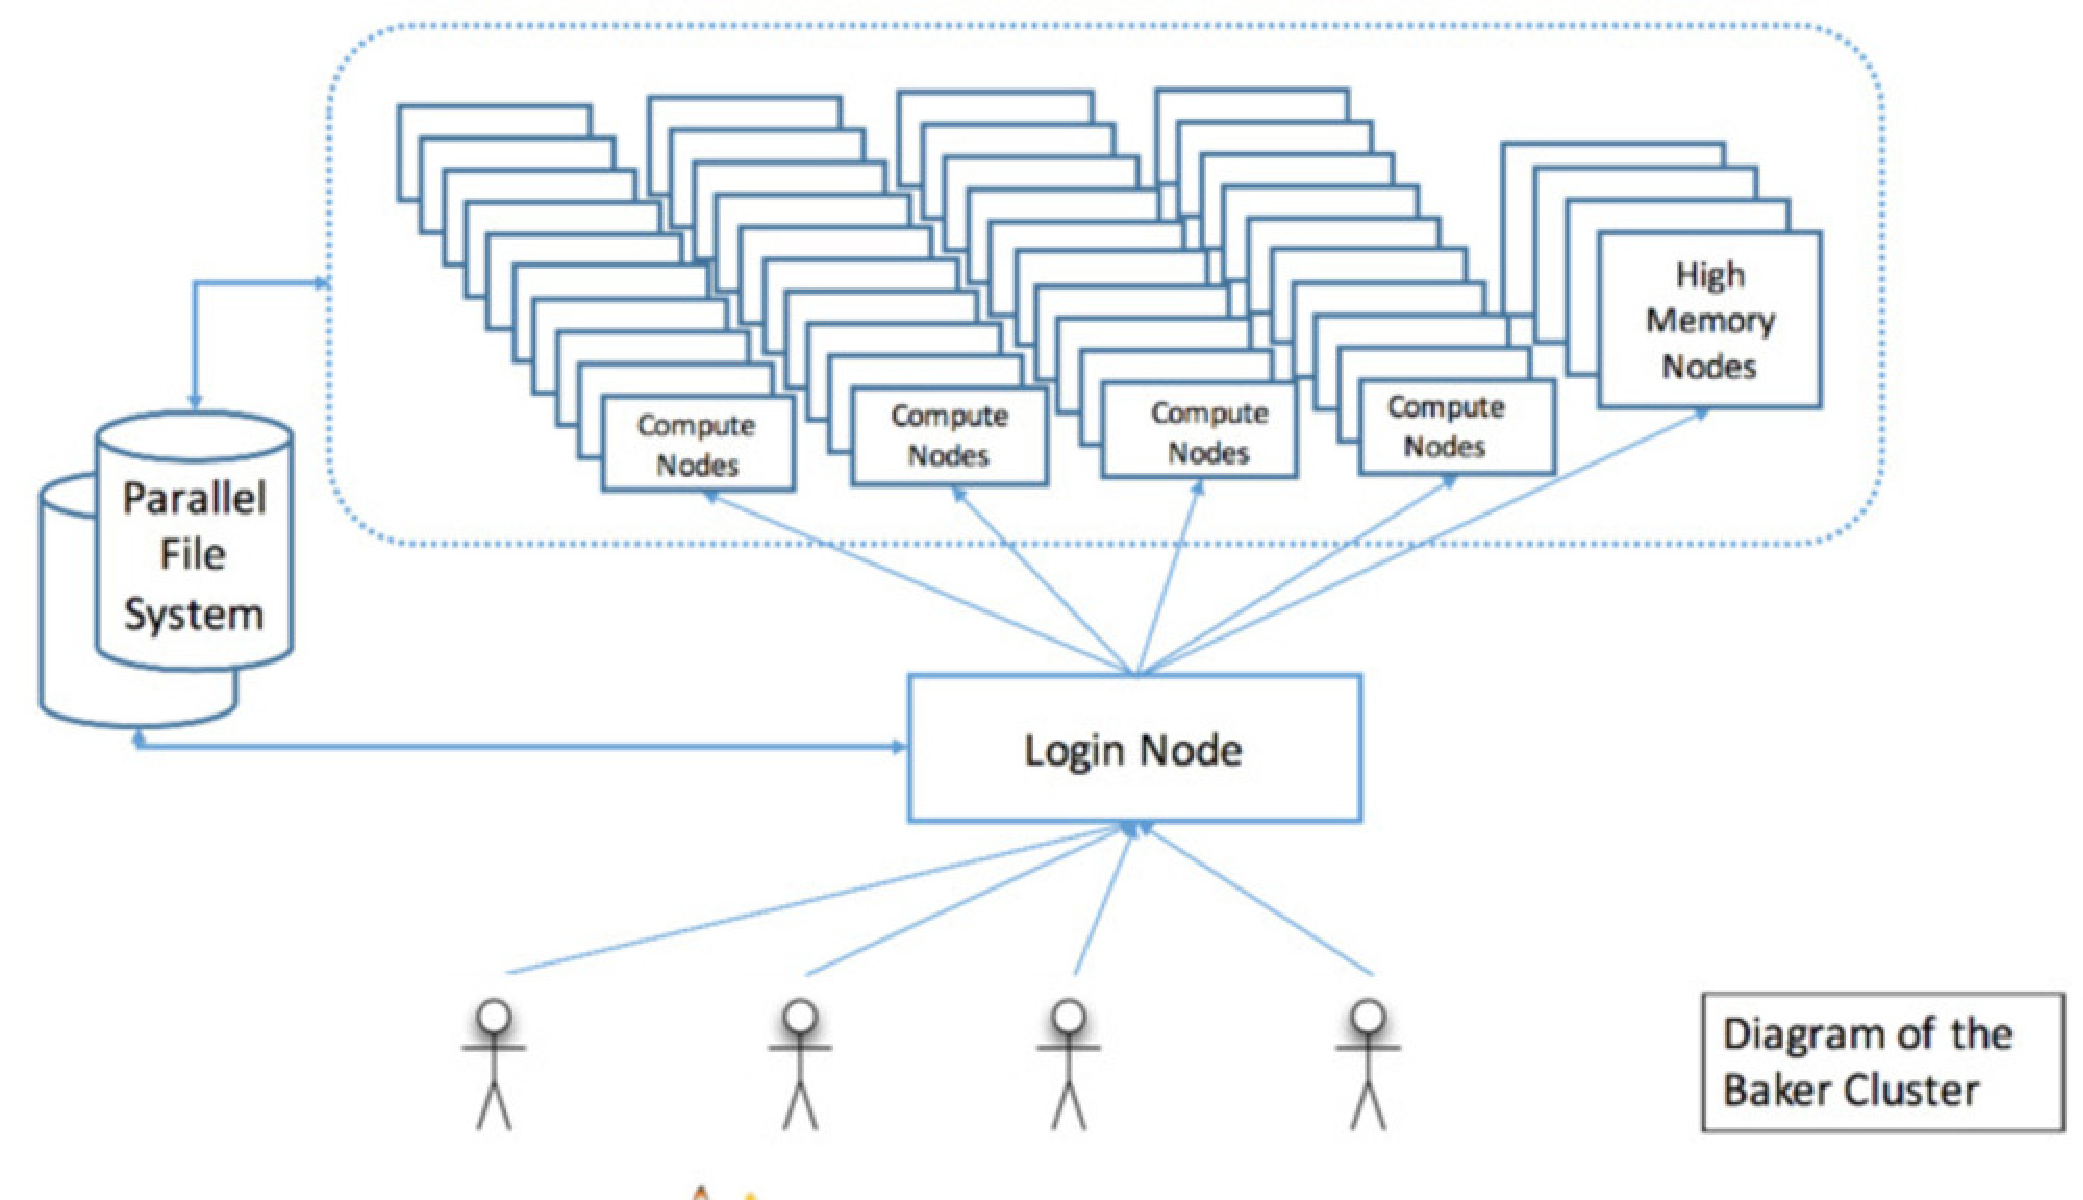
\includepdf{images/GPFS_File-eps-converted-to.pdf}
    %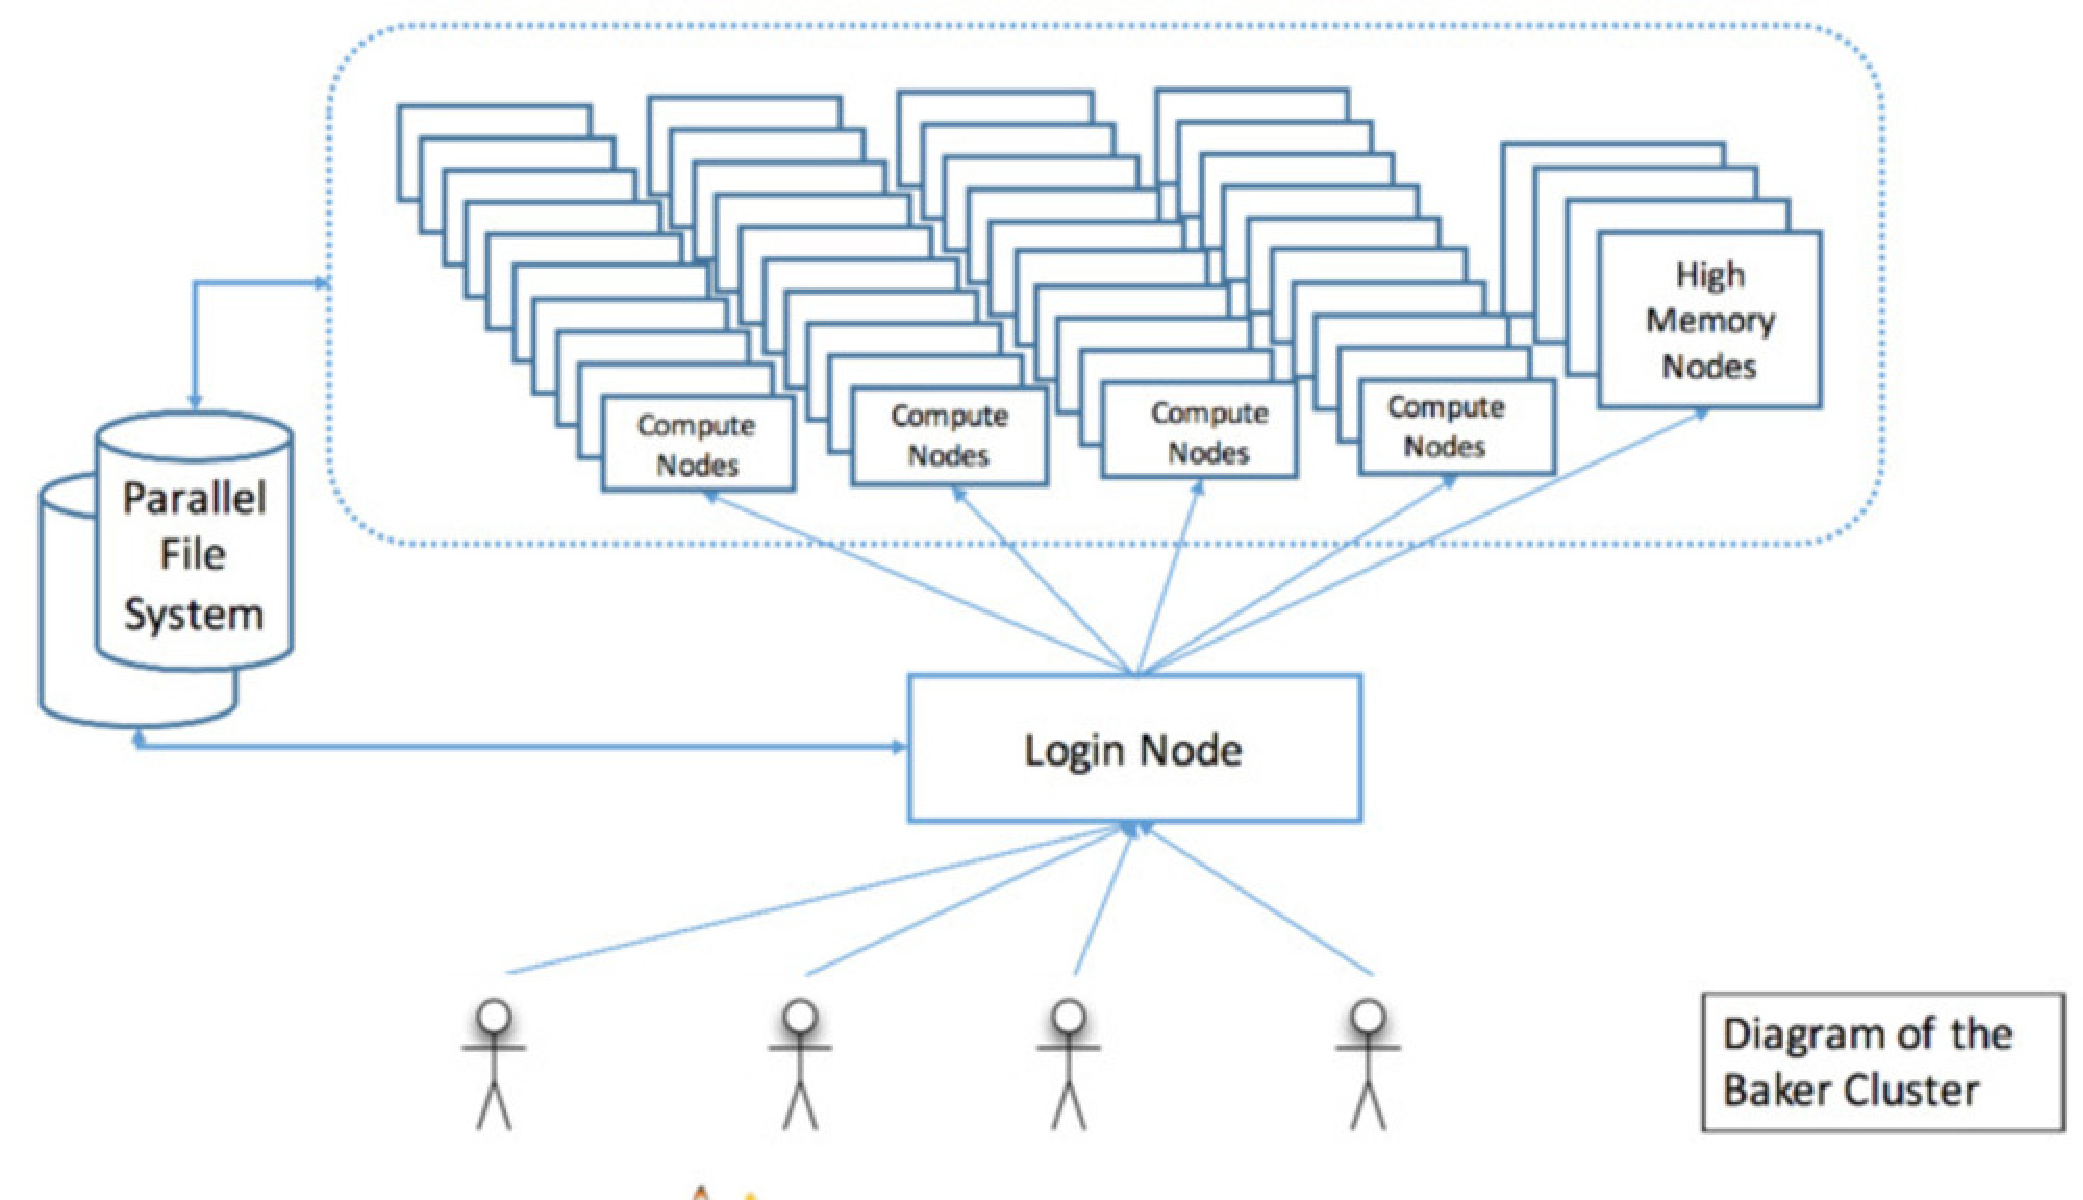
\includepdf{images/GPFS_File-eps-converted-to.pdf}
    %\put(65, 70){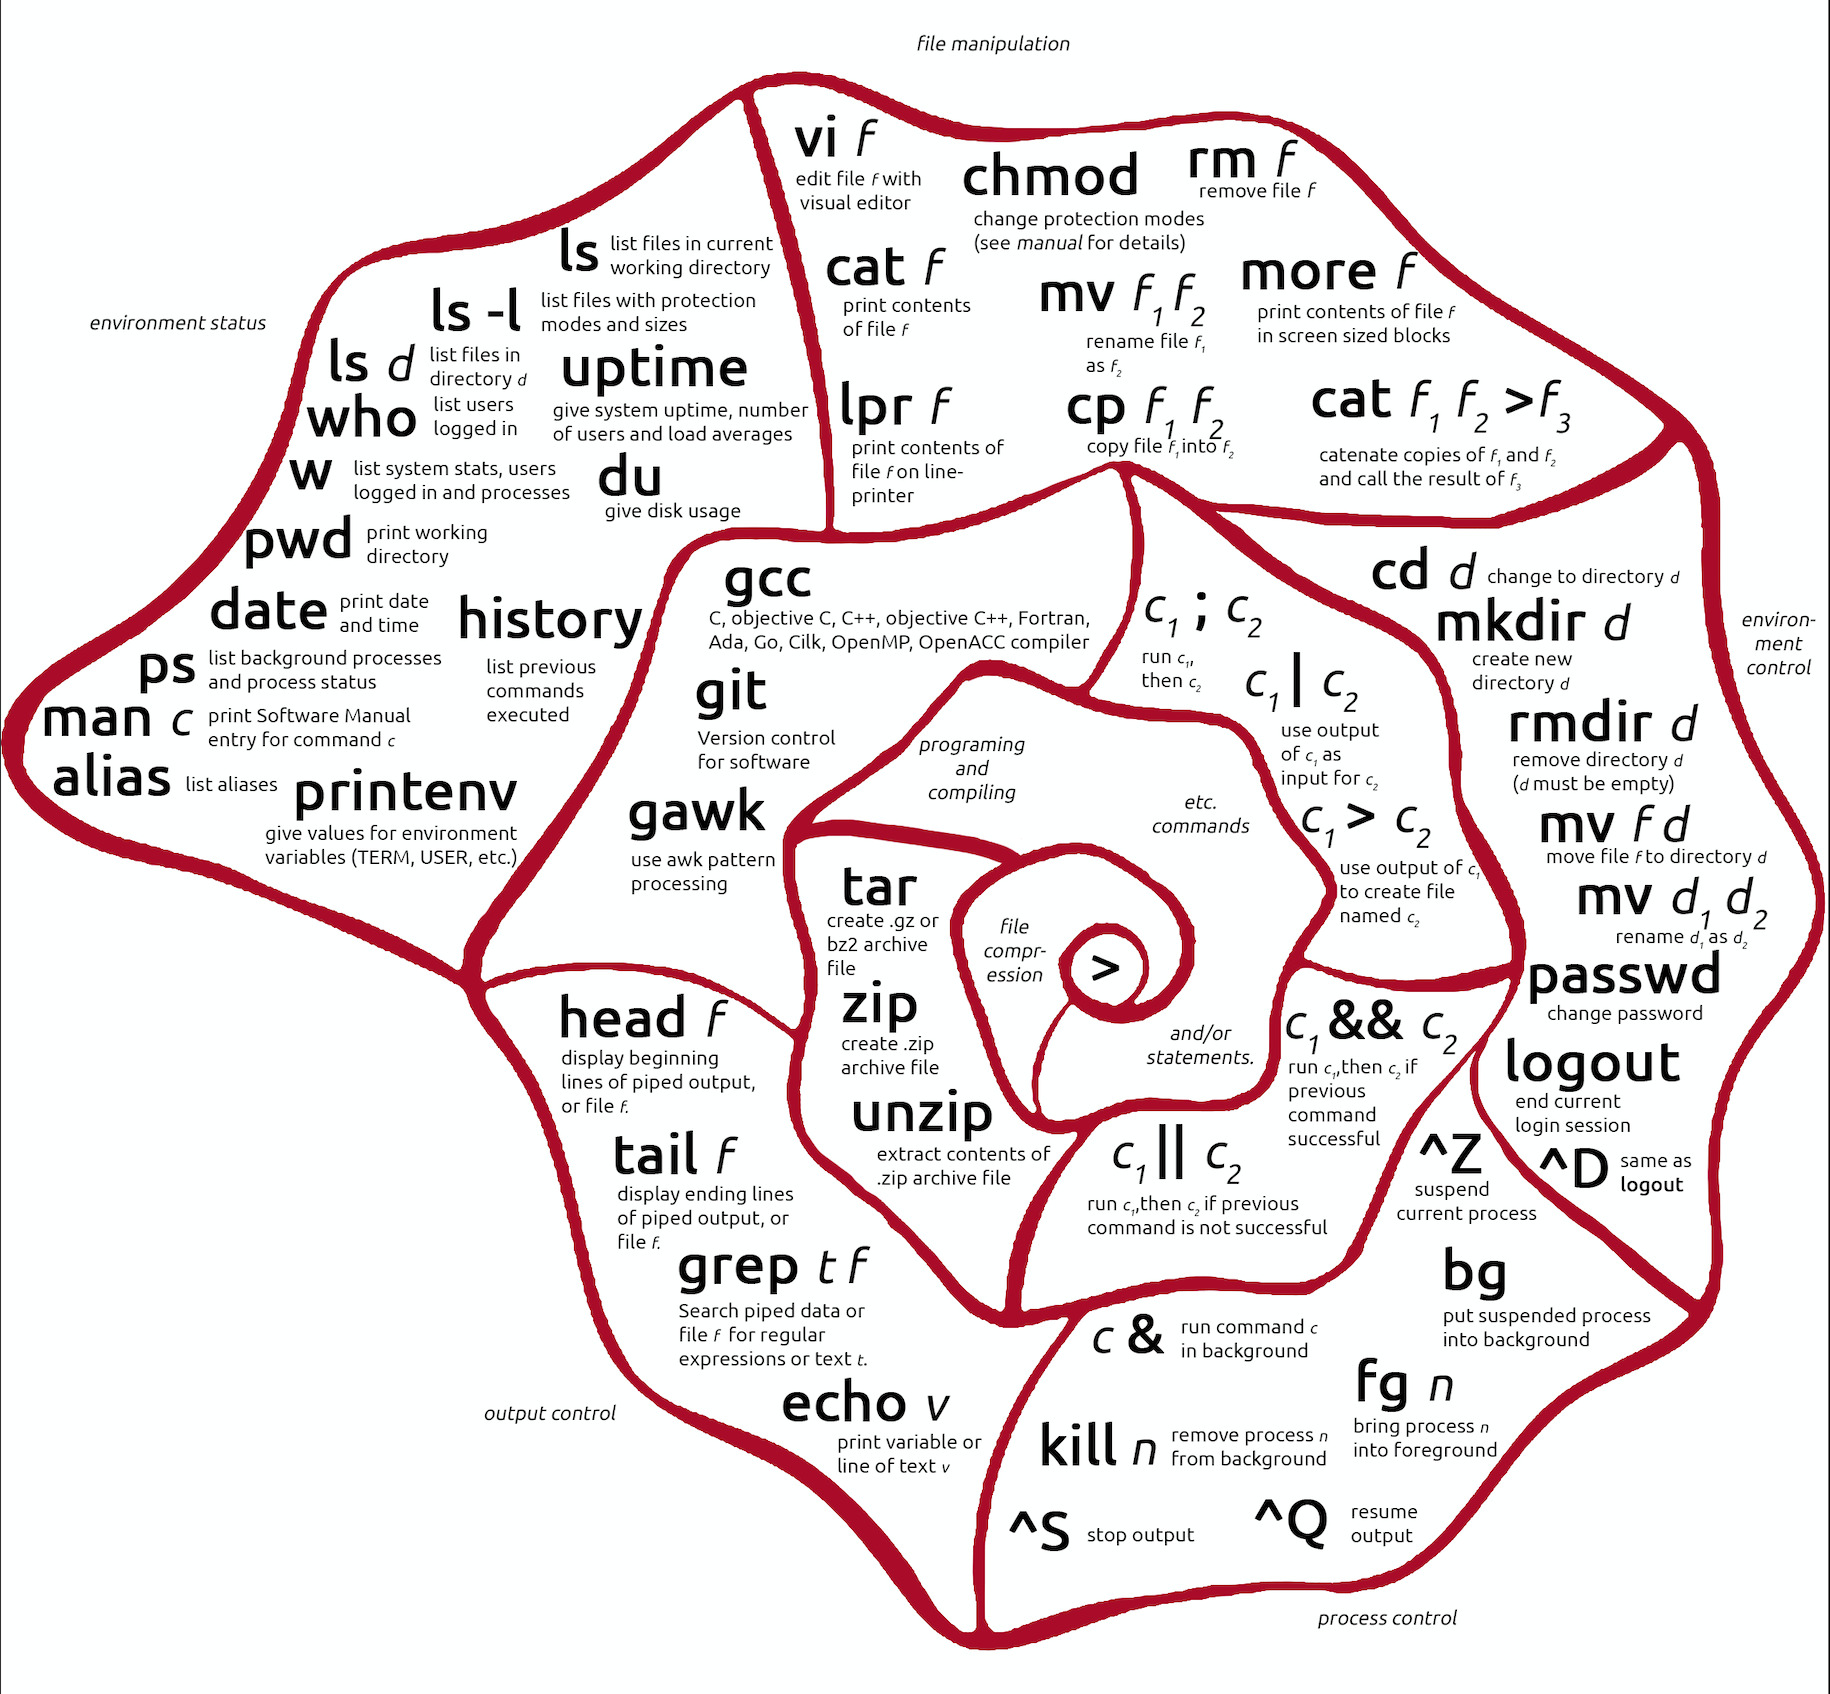
\includegraphics[height=2.5in]{images/linux-shell-small.jpg}}
    \end{picture}
\end{frame}
%\end{frame}


\begin{frame}
\frametitle{Text Editors}
\begin{itemize}
    \item \code{vim}   : Command line based
    \pause
    \bigskip
    \item \code{emacs} : Command line based
    \pause
    \bigskip
    \item \code{gedit} : Graphical  based
\end{itemize}
\end{frame}


\begin{frame}
\frametitle{Basic Commands}
\code{vim} - text editor
\bigskip
\begin{itemize}
    \item \code{vim $\sim$/tmp.txt}
    \bigskip
    \pause
    \item Command and Edit modes.
    \bigskip
    \pause
    \item \code{esc} to enter command mode
    \pause
    \bigskip
    \item \code{i} to enter edit mode
    \pause
    \bigskip
    \item To save, in command mode : \code{esc} \code{:w}
    \pause
    \bigskip
    \item To quit, in command mode : \code{esc} \code{:q}
\end{itemize}
\end{frame}


\begin{frame}
\frametitle{Basic Commands}
\code{ls} - List directories and files. E.g.
\bigskip
\begin{itemize}
    \item \code{ls /apps/opt/Python}
    \bigskip
    \pause
    \item \code{ls -l /apps/opt/Python} 
\end{itemize}
\end{frame}



\begin{frame}
\frametitle{Basic Commands}
\code{mkdir} - Make directories. E.g.
\bigskip
\begin{itemize}
    \item \code{mkdir $\sim$/newdir}
\end{itemize}
\end{frame}


\begin{frame}
\frametitle{Basic Commands}
\code{man} - prints user manual for command. E.g.
\bigskip
\begin{itemize}
    \item \code{man ls}
    \pause
    \bigskip
    \item Use \code{d} and \code{b} to navigate forward and back.
    \pause
    \bigskip
    \item Use \code{q} to quit
    \pause
    \bigskip
    \item Use \code{/somestring} to search for \code{somestring} within the man page.
\end{itemize}
\end{frame}


\begin{frame}
\frametitle{Basic Commands}
\code{cd}- Change directory. E.g.
\bigskip
\begin{itemize}
    \item \code{cd $\sim$/newdir}
    \pause
    \bigskip
    \item \code{cd}
    \pause
    \bigskip
    \item \code{cd ..}
    \pause
    \bigskip
    \item \code{cd $\sim$} 
\end{itemize}
\end{frame}


\begin{frame}
\frametitle{Basic Commands}
\code{pwd}- print working directory. E.g.
\bigskip
\begin{itemize}
    \item \code{pwd}
\end{itemize}
\end{frame}


%\begin{frame}
%\frametitle{Basic Commands}
%\code{touch}- Create empty file. E.g.
%\bigskip
%\begin{itemize}
%    \item \code{touch $\sim$/file.txt}
%\end{itemize}
%\end{frame}


\begin{frame}
\frametitle{Basic Commands}
\code{mv}- move file or rename file. E.g.
\bigskip
\begin{itemize}
    \item \code{mv $\sim$/file.txt $\sim$/file2.txt}
\end{itemize}
\end{frame}

\begin{frame}
\frametitle{Basic Commands}
\code{cp}- copy files or directories
\bigskip
\begin{itemize}
    \item \code{cp $\sim$/file2.txt $\sim$/file3.txt}
    \pause
    \bigskip
    \item \code{cp -r $\sim$/newdir $\sim$/newdir2}
\end{itemize}
\end{frame}


\begin{frame}
\frametitle{Basic Commands}
\code{rm}- delete files or directories. Be Careful. E.g.
\bigskip
\begin{itemize}
    \item \code{rm $\sim$/file.txt}
    \pause
    \bigskip
    \item \code{rm -r $\sim$/newdir}
\end{itemize}
\end{frame}


\begin{frame}
\frametitle{Basic Commands}
\code{cat}- concatenate files. E.g.
\bigskip
\begin{itemize}
    \item \code{cat /reference/README.txt}
\end{itemize}
\end{frame}


\begin{frame}
\frametitle{Basic Commands}
\code{echo}- echo back string. E.g.
\bigskip
\begin{itemize}
    \item \code{echo "Hello World"}
\end{itemize}
\end{frame}


%\begin{frame}
%\frametitle{Permissions}
%\code{chmod}- Change permissions.
%E.g.
%\begin{itemize}
%    \item \code{ls -l $\sim$/Scratch/file.txt}, yields : 
%    \hspace{5mm} \code{-rw-r--r--  1 user group 0 Apr  5 09:01 file.txt}
%    \smallskip
%\end{itemize}
%\bigskip
%
%
%% http://www.texample.net/tikz/examples/beamer-arrows/
%% https://tex.stackexchange.com/a/83434/84495
%\begin{tikzpicture}[overlay]
%
%%\coordinate (G) at (2.3,6.1);
%\coordinate (A) at (1.15,1.3);
%\coordinate (AU) at (1.15,1.5);
%\coordinate (B) at (1.65,1.3);
%\coordinate (BU) at (1.8,1.5);
%%\coordinate (AB1) at (1.35,1.3);
%\coordinate (AB1) at (1.55,1.3);
%\coordinate (AB2) at (0.5,0.3);
%
%
%\coordinate (C) at (1.80,1.3);
%\coordinate (D) at (2.35,1.3);
%\coordinate (CD1) at (2.15,1.3);
%\coordinate (CD2) at (2.15,0.3);
%
%
%\coordinate (E) at (2.50,1.3);
%\coordinate (EU) at (2.50,1.5);
%\coordinate (F) at (3.0,1.3);
%\coordinate (F1) at (3.15,1.3);
%\coordinate (FU) at (3.15,1.5);
%\coordinate (EF1) at (2.75,1.3);
%\coordinate (EF2) at (3.60,0.4);
%
%\draw [red,<-<,ultra thick]    (A) to[out=0,in=0] (B);
%\draw [red,-]    (A) -- (AU);
%\draw [red,-]    (C) -- (BU);
%\draw [red,-,ultra thick]    (AB1) -- (AB2);
%\draw [blue,<-<,ultra thick]   (C) to[out=0,in=0] (D);
%\draw [blue,-,ultra thick]   (CD1) -- (CD2);
%\draw [black,<-<,ultra thick] (E) to[out=0,in=0] (F);
%\draw [black,-]    (E) -- (EU);
%\draw [black,-]    (F1) -- (FU);
%\draw [black,-,ultra thick,bend right] (EF1) to[out=0,in=0] (EF2);
%\node[draw,red] at (0,0) {you};
%\node[draw,blue] at (2.15,-0) {group};
%\node[draw,black] at (4.8, -0) {everyone else};
%\draw [red,-,ultra thick]    (0.5,0) -- (2.25,-0.6);
%\draw [blue,-,ultra thick]   (2.6,-0.25) -- (2.6,-0.6);
%\draw [black,-,ultra thick]  (3.5,-0.250) -- (2.8,-0.6);
%\end{tikzpicture}
%\bigskip
%\pause
%\begin{itemize}
%    \smallskip
%    \item \code{chmod 755 file.txt}
%    \pause
%    \bigskip
%    %\item \code{ls -l $\sim$/Scratch/file.txt}, yields : 
%    %\hspace{5mm} \code{-rwxr-xr-x  1 user group 0 Apr  5 09:01 file.txt}
%    \item {\small \code{-rwxr-xr-x  1 user group 0 Apr  5 09:01 file.txt}}
%\end{itemize}
%\pause
%
%\bigskip
%Explanation:
%\begin{itemize}
%    %\item First number is you.
%    %\item Second number is for your group (i.e. lab).
%    %\item Third number is for everyone else.
%    \item \code{r} = 4, \code{w} = 2, \code{x} = 1
%    \item \code{7} = \code{4} + \code{2} + \code{1} = read (\code{r}) + write (\code{w}) +  execute(\code{x})
%    \item \code{5} = \code{4} + \code{1} = read (\code{r}), execute(\code{x})
%\end{itemize}
%
%
%\end{frame}
%
%

%\begin{frame}
%\frametitle{Permissions}
%\code{chmod}- Change permissions.
%E.g.
%\begin{itemize}
%    \item \code{ls -l $\sim$/Scratch/file.txt}, yields : 
%    \hspace{5mm} \code{-rw-r--r--  1 user group 0 Apr  5 09:01 file.txt}
%    \smallskip
%    \item \code{chmod 755 somescript.sh}
%    \bigskip
%    \item \code{ls -l $\sim$/Scratch/file.txt}, yields : 
%    \hspace{5mm} \code{-rwxr-xr-x  1 user group 0 Apr  5 09:01 file.txt}
%\end{itemize}
%\bigskip
%
%Explanation:
%\begin{itemize}
%    \item First number is you.
%    \item Second number is for your group (i.e. lab).
%    \item Third number is for everyone else.
%    \item \code{r} = 4, \code{w} = 2, \code{x} = 1
%    \item \code{7} = \code{4} + \code{2} + \code{1} = read (\code{r}) + write (\code{w}) +  execute(\code{x})
%    \item \code{5} = \code{4} + \code{1} = read (\code{r}), execute(\code{x})
%\end{itemize}
%\end{frame}
%

\section{HPC}

\begin{frame}
\frametitle{HPC Cluster Architecture}
\begin{picture}(320,250)  %must be related to where it is centered
%\put(0, 70){\includegraphics[height=2.5in]{images/GPFS_File.eps}}
%\setbeamercolor{background canvas}{bg=}
%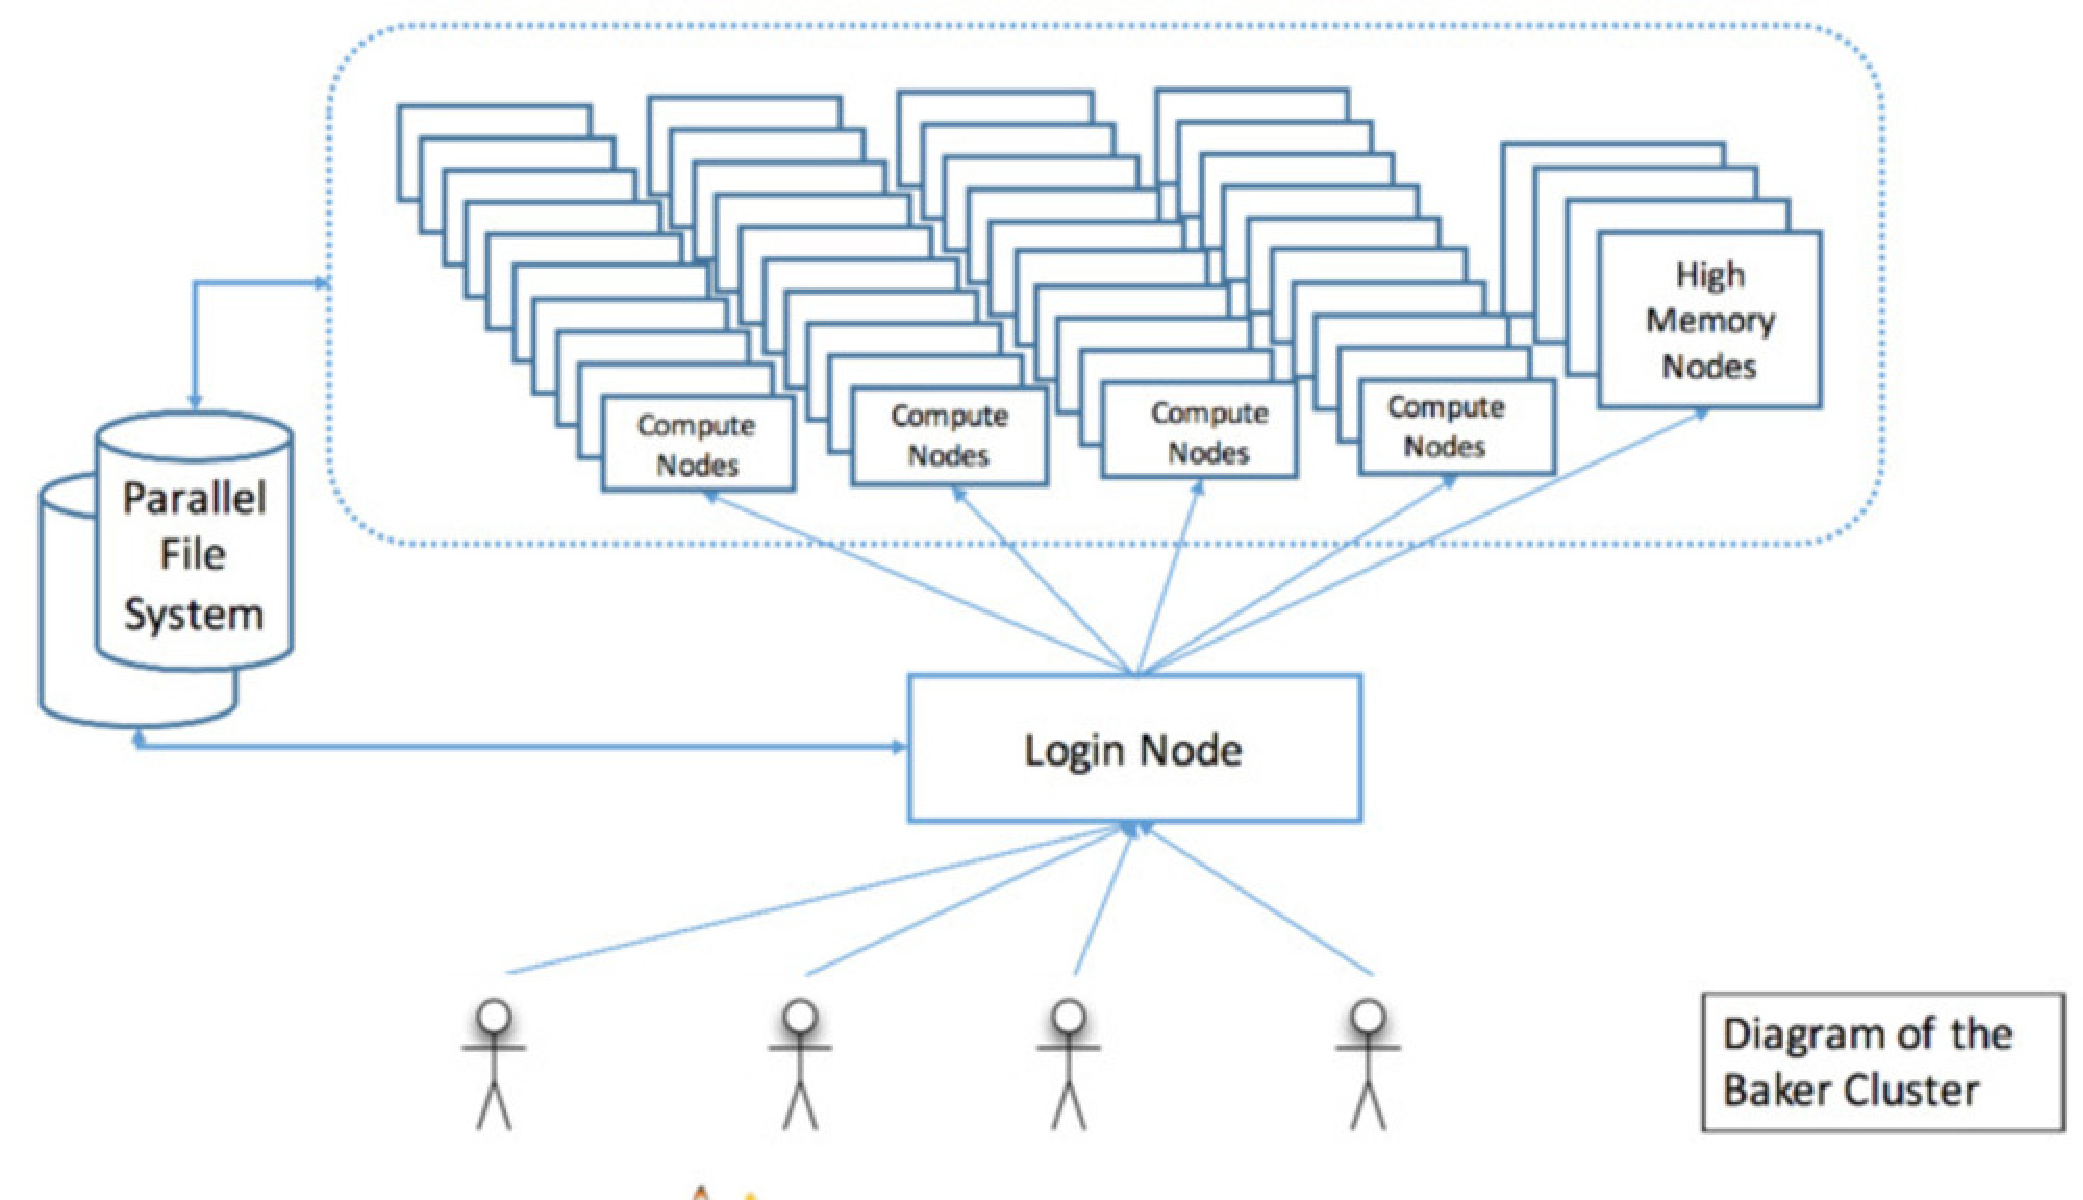
\includepdf{images/GPFS_File-eps-converted-to.pdf}
%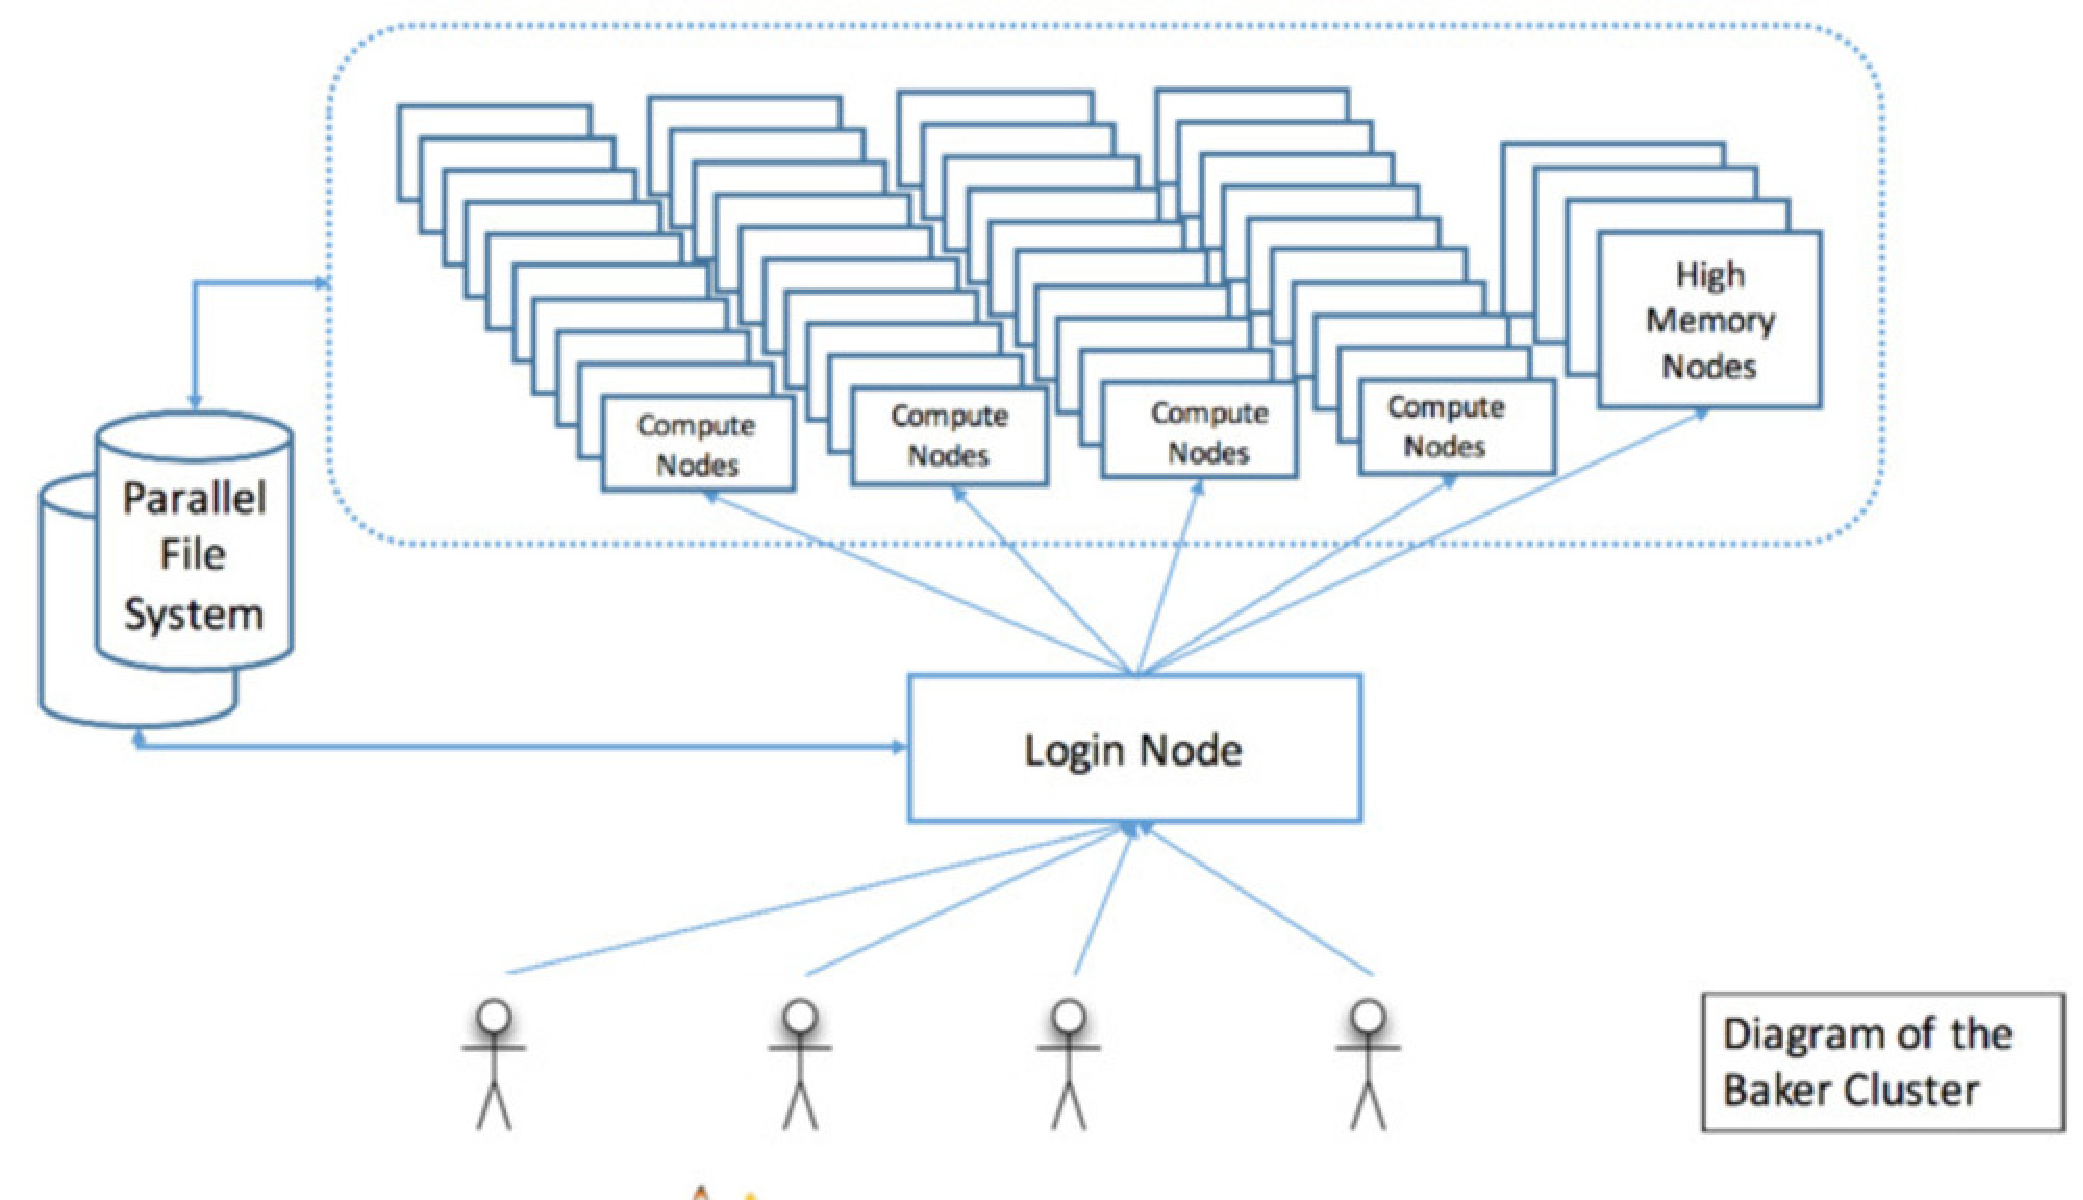
\includepdf{images/GPFS_File-eps-converted-to.pdf}
\put(65, 70){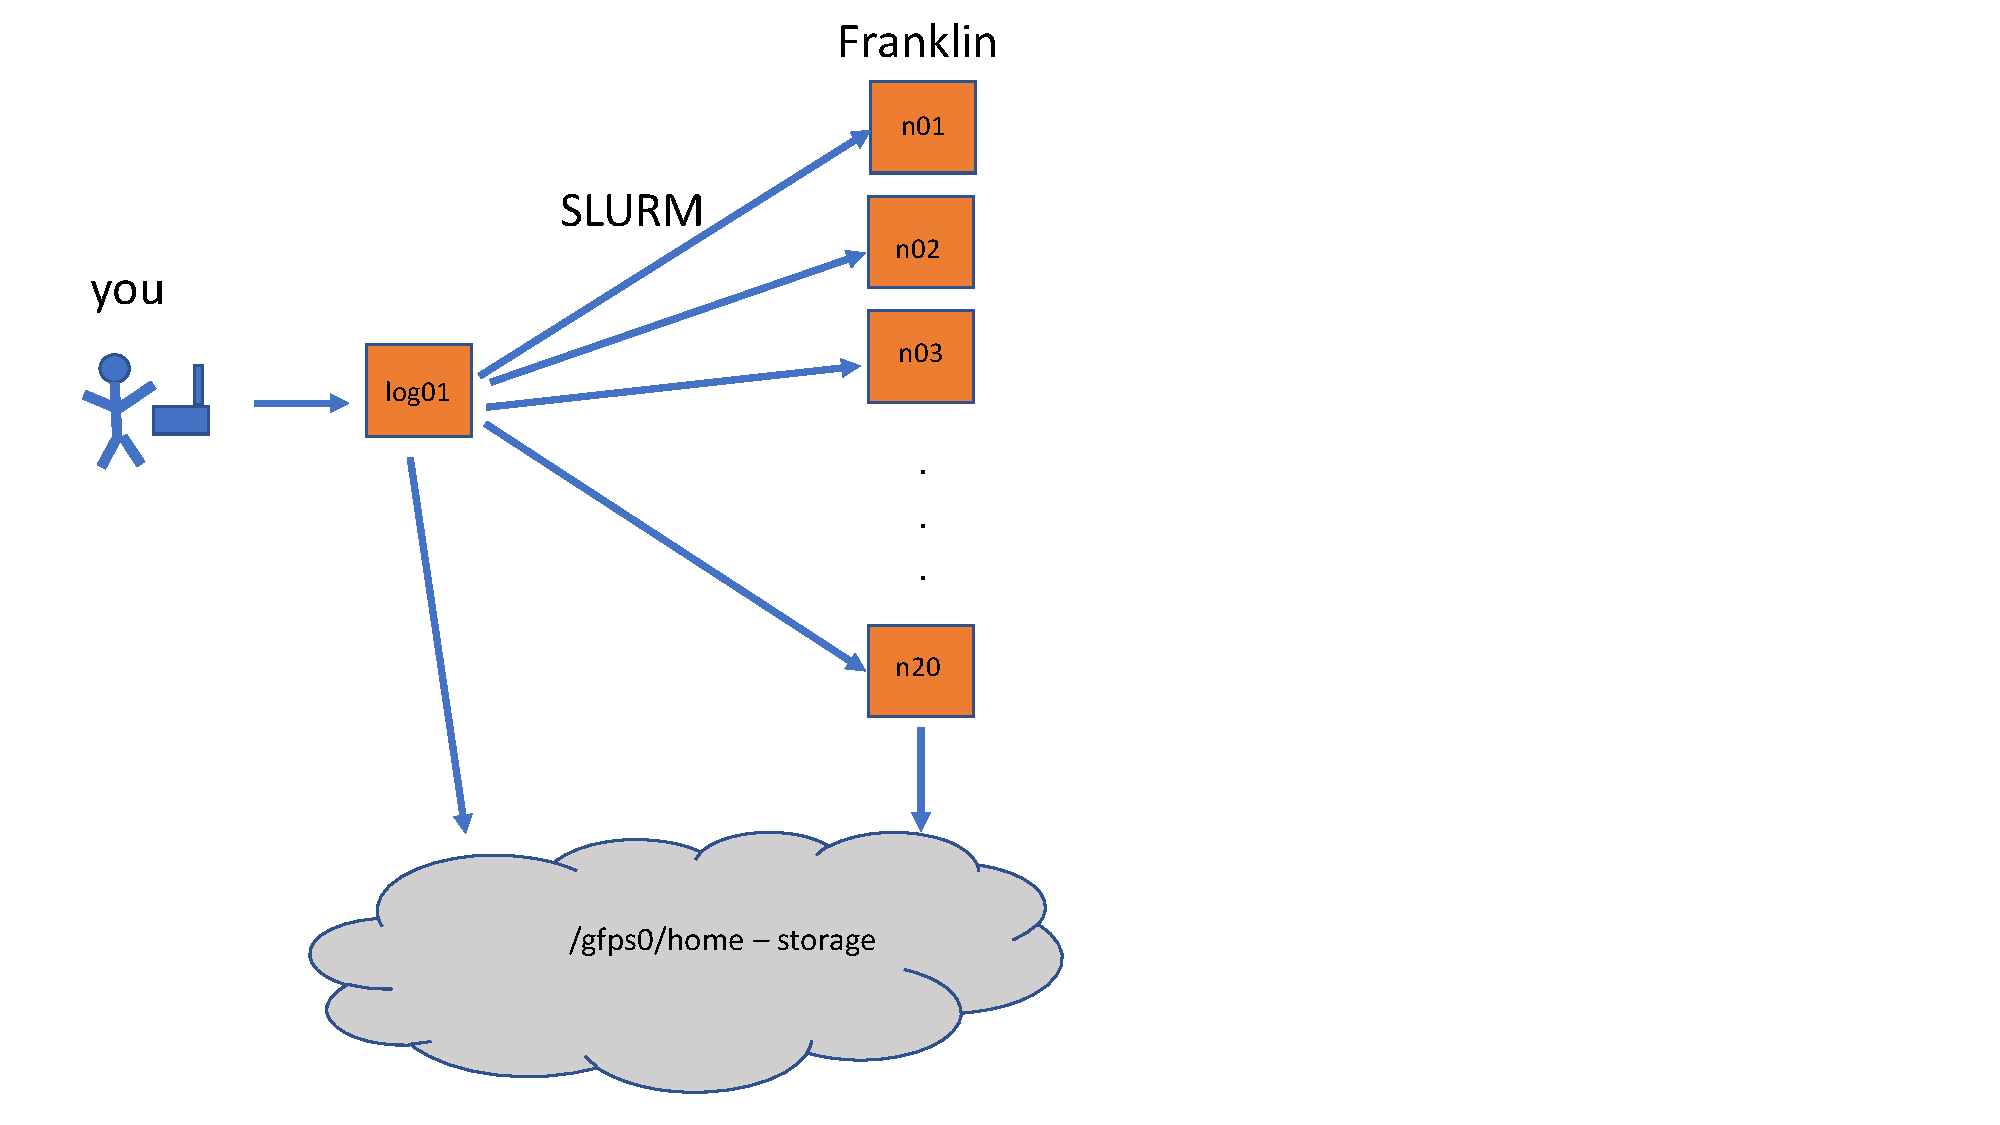
\includegraphics[height=2.5in]{images/franklin-cluster.pdf}}
\end{picture}
\end{frame}



\begin{frame}
\frametitle{What is SLURM?}
Need method for managing cluster resources.
\bigskip
\begin{itemize}
    \pause
    \item Enter SLURM - A Workload Manager
    \bigskip
    \pause
    \begin{enumerate}
        \item Permits efficient (and fair) utilization of Cluster resources.
        \pause
        \bigskip
        \item This is your interface with the computer cluster
    \end{enumerate}
\end{itemize}
\end{frame}




%\begin{frame}
%\frametitle{Slurm Concepts}
%\begin{itemize}
%    \item Job
%    \pause 
%    \begin{enumerate}
%        \item Primary way of requesting resources
%        \pause
%        \item Composed of one or more Steps
%    \end{enumerate}
%    \bigskip
%    \pause
%    \item Step
%    \begin{enumerate}
%        \item A way of dividing the resources allocated
%        \pause
%        \item Can be run serially or in parallel within a job
%        \pause
%        \item Composed of one or more Tasks
%    \end{enumerate}
%    \bigskip
%    \pause
%    \item Task
%    \begin{enumerate}
%        \item Composed of one or more CPUs
%    \end{enumerate}
%    \bigskip
%\end{itemize}
%\end{frame}



%\begin{frame}
%\frametitle{Franklin}
%A typical job on Franklin : 
%\bigskip
%\begin{itemize}
%    \item 1 Node 
%    \bigskip
%    \pause
%    \item 1 Task
%    \bigskip
%    \pause
%    \item Multiple CPUs
%    \bigskip
%    \pause
%\end{itemize}
%Complicated jobs may benefit from utilizing multiple steps and tasks, most jobs will not.
%\end{frame}
%

\begin{frame}
\frametitle{How to use Slurm?}
\begin{itemize}
    \item \code{sbatch} - Non-interactive bash script
    \bigskip
    \pause
    \item \code{srun} - Interactive sessions 
    \bigskip
\end{itemize}
\end{frame}



\begin{frame}
\frametitle{sbatch}
Examples of Usage:
\bigskip
\begin{itemize}
    \item \code{sbatch myscript.sh}
    \bigskip
    \pause
    \item \code{sbatch --cpus-per-task=20 myscript.sh}
    \bigskip
    \pause
    \begin{enumerate}
        \item NOTE : specifying 20 cores, will NOT magically make your script use 20 cores.
                     You will need to specify that within your shell script \code{myscript.sh}
    \end{enumerate}
    \pause
    \item \code{sbatch --gres=gpu myscript.sh}
    \bigskip
\end{itemize}
\end{frame}



\begin{frame}
\frametitle{sbatch}
Two ways to pass arguments to sbatch
\smallskip
\begin{itemize}
    \item Command line
        \smallskip
        \begin{enumerate}
            \item E.g. \code{sbatch OPTIONS myscript.sh}
            \pause
            \smallskip
            \item Popular \code{OPTIONS}
            \begin{enumerate}[a)]
                \item \code{--cpus-per-task=} 
                \pause
                \smallskip
                \item \code{--partition=himem}
                \pause
                \smallskip
                \item \code{--gres=gpu}
            \end{enumerate}
            \pause
            \smallskip
            \item Preempts options set in bash script
        \end{enumerate}
        \smallskip

    \pause
    \item In Bash Script, \code{myscript.sh}
        \pause
        \smallskip
        \begin{enumerate}
            \item Popular \code{OPTIONS}
            \pause
            \begin{enumerate}[a)]
                \item \code{\#SBATCH --cpus-per-task=} 
                \pause
                \smallskip
                \item \code{\#SBATCH --partition=himem}
                \pause
                \smallskip
                \item \code{\#SBATCH --gres=gpu}
            \end{enumerate}
        \end{enumerate}
\end{itemize}
\end{frame}



\begin{frame}[fragile]
\frametitle{sbatch}
Example \code{myscript.sh}: 
\begin{lstlisting}[backgroundcolor = \color{codegray}, language = Bash, showstringspaces=false]
    #!/bin/bash
    #SBATCH --cpus-per-task=10
    set -e
    echo "Hello World"
    sleep 30
\end{lstlisting}
\bigskip
\bigskip
Submit with \code{sbatch myscript.sh}
\end{frame}


\begin{frame}[fragile]
\frametitle{sbatch}
Output from batch script (\code{slurm-1795906.out}), will have some of the below information (some columns abbreviated for clarity)
\begingroup
\tiny
\begin{lstlisting}[backgroundcolor = \color{codegray}, language = Bash, showstringspaces=false]
Hello World
Job Statistics for 179:
       JobID   User Start End   Elapsed  MaxRSS   TotalCPU State Exit  NodeList
------------ ------ ----- --- --------- ------- ---------- ----- ---- ---------
         179 user01 ..... ...  00:00:00          00:00.009 COMPL  0:0    node01
   179.batch        ..... ...  00:00:00       0  00:00.008 COMPL  0:0    node01
  179.extern        ..... ...  00:00:00       0   00:00:00 COMPL  0:0    node01
CPU Efficiency: 0.00% of 00:00:00 core-walltime
\end{lstlisting}
\endgroup
\end{frame}


%\begin{frame}[fragile]
%\frametitle{sbatch}
%Himem partition allocation example \code{myscript\_himem.sh}: 
%\begin{lstlisting}[backgroundcolor = \color{codegray}, language = Bash, showstringspaces=false]
%    #!/bin/bash
%    #SBATCH --cpus-per-task=2
%    #SBATCH --partition=himem
%    set -e
%    echo "Hello World"
%    sleep 30
%\end{lstlisting}
%\bigskip
%\bigskip
%Submit with \code{sbatch myscript\_himem.sh}
%\end{frame}



%\begin{frame}[fragile]
%\frametitle{sbatch}
%Broken Example \code{myscript\_broken.sh}: 
%\begin{lstlisting}[backgroundcolor = \color{codegray}, language = Bash,showstringspaces=false]
%    #!/bin/bash
%    #SBATCH --cpus-per-task=2
%    #SBATCH --partition=himem
%    #SBATCH --mail-user=First.Last@gmail.com
%    #SBATCH --mail-type=FAIL,TIME_LIMIT_90
%    set -e
%    echo "I'm looking in the forbidden location"
%    ls /root/
%    echo "I never make it here"
%\end{lstlisting}
%\bigskip
%\bigskip
%Submit with \code{sbatch myscript\_broken.sh}
%\end{frame}


\begin{frame}
\frametitle{srun}
\code{srun} - Interactive allocation 
\bigskip
\begin{itemize}
    \item Use when needing to interactively run long processes. E.g.
        \begin{enumerate}
            \pause
            \item compiling
            \pause 
            \item developing and testing workflows
            \pause 
            \item downloading data
            \pause 
            \item GUI editors, e.g. RStudio
            \pause 
            \item Plotting, e.g. gnuplot, matplotlib
        \end{enumerate}
    \pause
    \item Example command : \code{srun --x11 --cpus-per-task=2 --pty bash}
        \pause
        \begin{enumerate}
            \item \code{--x11} option only needed for GUIs (e.g. RStudio)
            \pause
            \item For \code{--x11} to work, you must have X11 server installed
            \pause
            \begin{enumerate}[a)]
                \item Vcxsrv for Windows
                \pause
                \item XQuartz for Mac
            \end{enumerate}
        \end{enumerate}
    \pause
    \item \code{srun} takes all same command line options as \code{sbatch}
\end{itemize}
\end{frame}


\begin{frame}
\frametitle{Monitoring Jobs Progress}
There are several ways to monitor jobs progress.  
\bigskip
\begin{itemize}
    \item \code{squeue}
    \pause
    \bigskip
    \item \code{scontrol}
\end{itemize}
\end{frame}


\begin{frame}[fragile]
\frametitle{Monitoring Jobs Progress}
\code{squeue}, e.g. 
\begingroup
\tiny
\begin{lstlisting}[backgroundcolor = \color{codegray},showstringspaces=false]
   JOBID PARTITION          NAME     USER ST       TIME  NODES      CPUS NODELIST(REASON)
 1791312   general gromacs_test_   user01  R 9-21:30:30      1        20 node02
 1791313   general gromacs_test_   user01  R 9-21:30:09      1        20 node03
 1791316   general          his1   user01  R 9-21:28:56      1        20 node06
 1791317   general          his1   user01  R 9-21:28:53      1        20 node07
 1794106   general          test   user02  R 3-20:17:31      1        20 gpu03
 1794236   general          bash   user03  R 2-23:33:53      1         1 node01
\end{lstlisting}
\endgroup
\end{frame}



%\begin{frame}[fragile]
%\frametitle{Monitoring Jobs Progress}
%\code{scontrol}, e.g. \code{ scontrol show jobid 1794106}
%\begingroup
%\tiny
%\begin{lstlisting}[backgroundcolor = \color{codegray},showstringspaces=false]
%JobId=1794106 JobName=test
%   UserId=user02(600) GroupId=group01(1181939003) MCS_label=N/A
%   Priority=28575 Nice=0 Account=gdpairlab QOS=normal
%   JobState=RUNNING Reason=None Dependency=(null)
%   Requeue=1 Restarts=0 BatchFlag=1 Reboot=0 ExitCode=0:0
%   RunTime=3-20:25:41 TimeLimit=7-00:00:00 TimeMin=N/A
%   SubmitTime=2019-04-15T12:30:01 EligibleTime=2019-04-15T12:30:01
%   StartTime=2019-04-15T12:30:02 EndTime=2019-04-22T12:30:02 Deadline=N/A
%   PreemptTime=None SuspendTime=None SecsPreSuspend=0
%   LastSchedEval=2019-04-15T12:30:02
%   Partition=general AllocNode:Sid=qmaster01:20116
%   ReqNodeList=gpu03 ExcNodeList=(null)
%   NodeList=gpu03
%   BatchHost=gpu03
%   NumNodes=1 NumCPUs=20 NumTasks=1 CPUs/Task=20 ReqB:S:C:T=0:0:*:*
%   TRES=cpu=20,mem=120G,node=1,billing=20,gres/gpu=1
%   Socks/Node=* NtasksPerN:B:S:C=0:0:*:* CoreSpec=*
%   MinCPUsNode=20 MinMemoryCPU=6G MinTmpDiskNode=0
%   Features=(null) DelayBoot=00:00:00
%   Gres=gpu:1 Reservation=(null)
%   OverSubscribe=OK Contiguous=0 Licenses=(null) Network=(null)
%   Command=/gpfs0/home/group01/user02/ram_test/start_gtn.sh
%   WorkDir=/gpfs0/home/group01/user02/ram_test
%   StdErr=/gpfs0/home/group01/user02/ram_test/test_1794106.out
%   StdIn=/dev/null
%   StdOut=/gpfs0/home/group01/user02/ram_test/test_1794106.out
%   Power=
%\end{lstlisting}
%\endgroup
%\end{frame}




%\begin{frame}[fragile]
%\frametitle{Homework 1 - Illustrating jobs, steps and tasks}
%Consider the following scripts
%
%\medskip
%\code{step.sh}
%\begingroup
%\small
%\begin{lstlisting}[backgroundcolor = \color{codegray},showstringspaces=false, language=Bash]
%#!/bin/bash
%#SBATCH --cpus-per-task=10
%#SBATCH --tasks-per-node=2
%srun --ntasks=1 bash other.sh first_step &
%srun --ntasks=1 bash other.sh second_step &
%wait
%\end{lstlisting}
%\endgroup


%\medskip
%\code{other.sh}
%\begingroup
%\small
%\begin{lstlisting}[backgroundcolor = \color{codegray},showstringspaces=false, language=Bash]
%#!/bin/bash
%date
%echo "Hello from $1"
%sleep 30
%echo "World from $1"
%date
%\end{lstlisting}
%\endgroup
%\end{frame}
%
%

%\begin{frame}
%\frametitle{Homework 1 - Illustrating jobs, steps and tasks}
%\begin{itemize}
%    \item Submit job \code{step.sh}
%    \bigskip
%    \item Remove the \code{\&} at the end of the lines. What happens?
%    \bigskip
%    \item Remove the \code{\&} at the end of the lines along with \code{wait}. What happens?
%    \bigskip
%    \item Remove the \code{--ntasks=1}, along with \code{\&} and \code{wait}. What happens?
%    \bigskip
%    \item Try different combinations.
%\end{itemize}
%\end{frame}

\begin{frame}
\frametitle{Homework}
Create a bash script that says ``Hello World" and submit it to the cluster.

\bigskip

\emph{HINT}, you'll need to add $\code{\#^^21/bin/bash}$ at the top of your script
\end{frame}


\begin{frame}
\frametitle{References}
\begin{itemize}
    \item \chref{https://www.opensourceforu.com/2020/03/reasons-to-use-linux/}{Ten Reasons why we should use Linux}
    \item \chref{https://www.extremetech.com/extreme/155392-international-space-station-switches-from-windows-to-linux-for-improved-reliability}{ISS switches from Windows to Linux, for improved reliability}
    \item \chref{https://medium.com/geekculture/how-to-stop-windows-10-from-spying-on-you-b071134a11f6}{How to Stop Windows 10 From Spying on You}
    \item \chref{https://washingtonsblog.com/microsoft-programmed-in-nsa-backdoor-in-windows-by-1999/}{NSA Built Back Door In All Windows Software by 1999}
    \item \chref{https://security.stackexchange.com/a/96715/94605}{How does Windows 10 allow Microsoft to spy on you?}
    \item \chref{https://medium.com/geekculture/how-linux-helped-us-land-on-mars-a2ceb54cf6e}{How Linux Helped Us Land On Mars}
    \item \chref{https://www.lbto.org/software-eng-202102.html}{Large Binocular Telescope Software}
    \item \chref{https://www.skatelescope.org/software-and-computing/}{SKA Software and Computing}
\end{itemize}
\end{frame}


\begin{frame}
\frametitle{Images}
\begin{itemize}
    \item \chref{https://www.nasa.gov/sites/default/files/thumbnails/image/spacestationfaqs.jpg}{ISS - Public Domain}
    \item \chref{https://home.cern/news/news/accelerators/lhc-rocks-seesaw-model}{LHC - Fair Use}
    \item \chref{https://mars.nasa.gov/resources/26253/perseverances-selfie-at-rochette/}{Perserverance - Public Domain}
    \item \chref{ https://commons.wikimedia.org/w/index.php?curid=32980017}{LBT By Mohamed Osama AlNagdy - Copyrighted free use}
    \item \chref{https://www.skatelescope.org/news/green-light-for-ska-construction/}{SKA - Public Domain}
    \item \chref{https://www.csm.ornl.gov/PR/PR2006/hpc-07-21-06.html}{Climate Modeling - Fair Use}
    \item \chref{https://external-preview.redd.it/M11dk9cVQ4nHdBHWPGR0w4-2p\_S0CRTuiFRWNkM3Bks.png?auto=webp&s=021bc36b5e08fe70156ac635a9530fdc438acf4a}{Linux Shell by JaceTheSaltScultor - Fair Use}
\end{itemize}
\end{frame}

\end{document}

